% ****** Start of file apssamp.tex ******
%
%   This file is part of the APS files in the REVTeX 4.1 distribution.
%   Version 4.1r of REVTeX, August 2010
%
\documentclass[reprint,%article
 %,
%superscriptaddress,
%groupedaddress,
%unsortedaddress,
%runinaddress,
%frontmatterverbose, 
%preprint,
%showpacs,preprintnumbers,
%nofootinbib,
%nobibnotes,
%bibnotes,
 amsmath,amssymb,
 aps,
%pra,
%prb,
%rmp,
%prstab,
%prstper,
%floatfix,
]{revtex4-1}

\usepackage{xcolor}

\usepackage{graphicx}% Include figure files
\usepackage{dcolumn}% Align table columns on decimal point
\usepackage{bm}% bold math
\usepackage{appendix}
\usepackage{subcaption}
%\usepackage{subfloat}
%\usepackage{hyperref}% add hypertext capabilities
%\usepackage[mathlines]{lineno}% Enable numbering of text and display math
%\linenumbers\relax % Commence numbering lines

%\usepackage[showframe,%Uncomment any one of the following lines to test 
%%scale=0.7, marginratio={1:1, 2:3}, ignoreall,% default settings
%%text={7in,10in},centering,
%%margin=1.5in,
%%total={6.5in,8.75in}, top=1.2in, left=0.9in, includefoot,
%%height=10in,a5paper,hmargin={3cm,0.8in},
%]{geometry}https://www.overleaf.com/project/5ba0361831a91c7b3990c0d7
 \usepackage{natbib}
 
\begin{document}

\preprint{APS/123-QED}

\title{DRAFT- Rotation Curve Fitting Model }% Force line breaks with \\
%\thanks{ Thanks Jesus}%

% Find out if Joe and Noah still want to be on this paper%

 

\author{Sophia Natalia Cisneros}
 \affiliation{ Department of Astronomy,  
 University of Washington}
 % \email{sophia.cisneros@du.edu}
  \author{Richard Ott}%
 \email{rich.ott@EMAIL.com}
\affiliation{Gotta get that}%Tech dudes \textbackslash\textbackslash
%}
 \author{ Meagan Crowley}
\email{ }
\affiliation{NREL}%
 \author{ Amy Roberts}
\email{ }
\affiliation{CU Denver}%
\author{Marcus Paz}
\author{Zaneeyiah Brown}
\author{Landon Joyal}
\author{Roberto Real Rico}
\author{Elizabeth Gutierrez-Gutierrez}
\author{ Phong Pham}
\author{Zac Holland}
\author{Amanda Livingston}
\author{Lily Castrellon}
\author{Shanon Rubin}
\author{Aaron Ashley}
\author{Dillon Battaglia}
%\affiliation{UMass Boston% with \\
%&}%
%
%\affiliation{%
%University Denver
%}%

%\affiliation{%
%UC Davis
%
%%\\author{J.G. O'Brien}%
%\affiliation{%
%Wentworth Institute of Technology 
% 

 
\date{\today}% It is always \today, today,
             %  but any date may be explicitly specified
\begin{abstract}
{\color{teal}  EDIT }
The flat-rotation curve problem of spiral galaxies is generally resolved by the introduction of new physics. Either
 Dark Matter theories introduce new particles or Modified Newtonian Dynamics a new gravitational scale. In both paradigms,     Doppler shifted spectra     are interpreted by a Lorentz boost   velocities between inertial frames. 
 We   instead phrase  excesses in Doppler shifted   spectra  as relative gravitational frame effects due to our Milky Way. 
     This   approach  employs  a new technique, but no new physics, and more naturally explains why galaxies smaller than the Milky Way have rotation curves which ascend past the optical light, and those larger than the Milky Way fall, though not in a Keplerian sense.  
 In this paper we demonstrate the efficacy of  this    frame dependent approach  on  the SPARC sample of 174 galaxies (Spitzer  Photometry and Accurate Rotation Curves) as  previously reported for Modified Newtonian Dynamics  fits(CITE).  

\begin{description}
\item[Usage]
Secondary publications and information retrieval purposes.
\item[PACS numbers]
May be entered using the \verb+\pacs{#1}+ command.
\item[Structure]
You may use the \texttt{description} environment to structure your abstract;
use the optional argument of the \verb+\item+ command to give the category of each item. 
\end{description}
\end{abstract}

\pacs{Valid PACS appear here}% PACS, the Physics and Astronomy
                             % Classification Scheme.
%\keywords{Suggested keywords}%Use showkeys class option if keyword
                              %display desired
\maketitle

%\tableofcontents
%%%%%%NOTES TO DO
%%%make labels for figure axes. remove orange line through the data



%%%%%%
%%%%%%%%
%%%%%%
%%%%%%%
%%%%%%
%%%%%%
\section{Introduction  \label{sec:uno}}
%DARK MATTER

 The flat-rotation curve problem of spiral galaxies   arises from two   observations of light, photometry and spectra, both assumed proxies for mass. The first observation is Photometry,  the measure of a galaxy's total light which is assumed to trace baryonic mass,  and yields Keplerian velocities which fall-off   outside of the stars. 
    The second observations is Doppler shifted spectra, which is interpreted as   relative frame motion between two inertial frames, and yield velocities which do not decrease past the stars.
 It is assumed that since both observations are proxies for mass, then  there must be a 
    a missing or dark matter problem  (Fig.~\ref{fig:NGC2403}).   Hence,  the     flat-rotation curve problem was born\cite{Rub},\cite{Bosma},\cite{Zwick} as one of the first indicators of a missing mass problem in cosmology. Since that time, many different physics problems in the standard concordance model of cosmology  $\lambda$CDM have been attributed to missing mass. In this work we address only that of the flat-rotation curve problem because  the frame dependent symmetry we invoke is particularly clear. We assume as well that many of the other problems usually attributed to dark matter can be evaluated in a more complete cosmology.
    
 
    There exist problems with the dark matter solution in rotationally supported galaxies due to a conflict between the underpinning theory and the observations.  Dark matter theory is built on classical gravity,   but yet has  to accommodate the empirical fact that smaller galaxies require proportionally larger dark matter halos than large galaxies. This trend is called the Universal Rotation Curve  (See Fig.~\ref{fig:URC}).
     In classical Einstein gravity, larger mass concentrations are more successful at mass accretion. Dark matter accommodates this paradox  by fine-tuning (CITE). In this paper, we remove this paradox by  viewing the trend in rotation curves with respect to the Milky Way (SEE FIGURE) as evidence for a frame-dependent approach (CITE).  
    
  The leading   alternative to dark matter    is called Modified Newtonian Dynamics (MOND) \cite{Milgrom}.  In MONDian thought, the flat-rotation curve problem is due to a changing gravitational acceleration scale on the vast distances of galaxies.  
 MOND leverages the curious correlation between dark and luminous matter \cite{McGaugh_2014} to state that baryonic mass is the only mass, but that the Doppler shifted velocities  are hinting at new gravitational physics on the length scales of galaxies and groups of galaxies.  This approach  is remarkably successful in predicting  rotation curves  across a diverse range  of galaxies,   using only the inputs of the luminous mass and a free parameter for the   acceleration scale \cite{McGaugh2016RAR}. 
 Notably, roughly the same acceleration threshold works for nearly all galaxies. In our frame-dependent approach, we interpret   MOND's single-valued acceleration scale as accurately describing the effects of our Milky Way on our observations, and when extended to a semi-relativistic framework for weak fields, the concept of changing accelerations naturally transitions to relative curvatures. 
 
    
 \begin{figure}[h!]
%\scalebox{0.25075}%
      \centering
      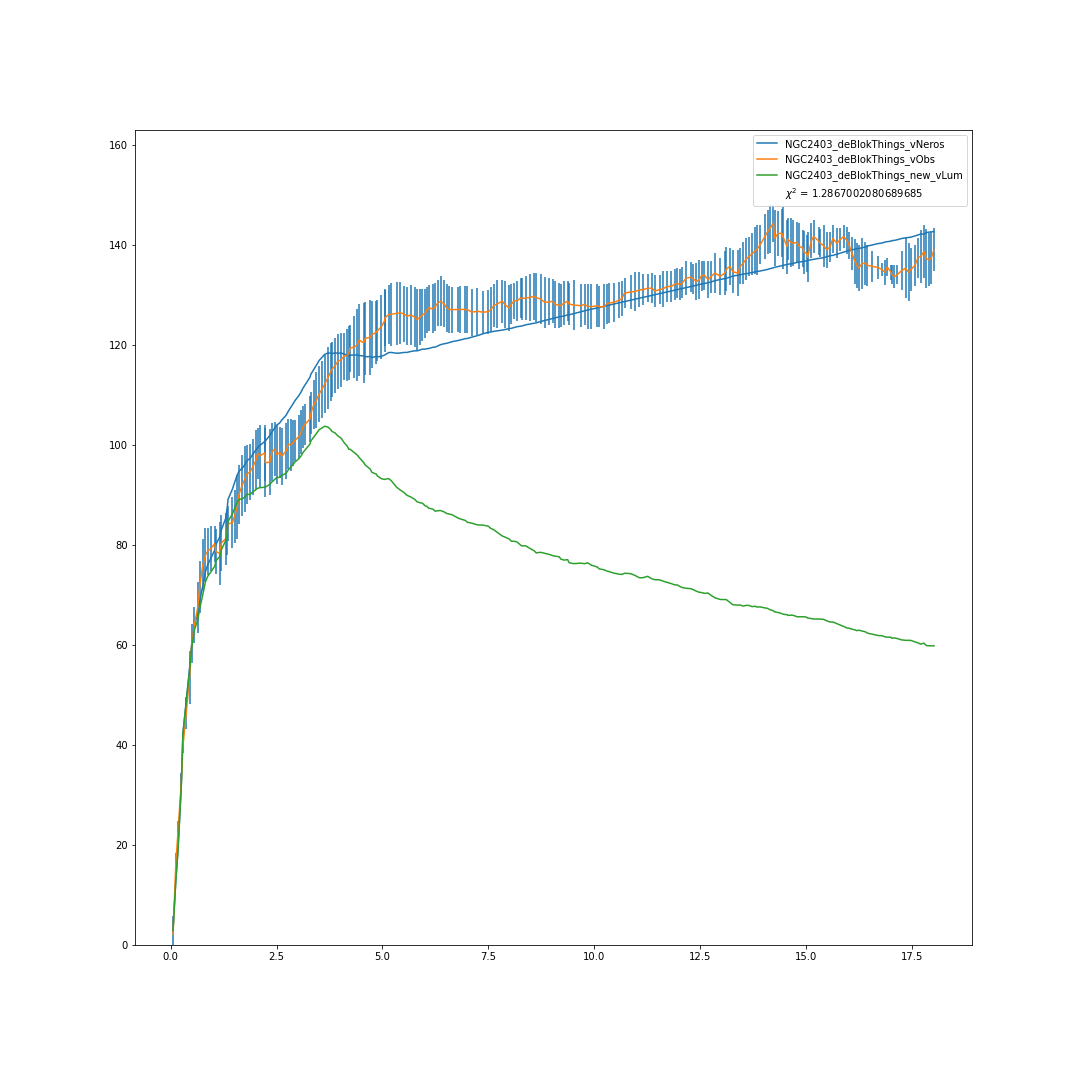
\includegraphics[width=\linewidth]{NGC2403_deBlokThings_XueSofue}
      \caption{Rotation Curve of NGC 2403 \cite{Blok1},  Rotation curve data points blue dots with  error bars, expected Keplerian velocity from luminous mass estimated by   green line, fitted with the RCFM presented here, blue line. }
      \label{fig:NGC2403}
  \end{figure}
  
  %MOND  %MONDian       
 
 
  Attempts at extending MONDian reasoning into the relativistic regime have given rise to a new theory of gravity called TeVeS, but remains  a modification to the well tested Einstein gravity  \cite{PhysRevD.70.083509}.
 Here we will propose a more conservative approach, in which excesses in Doppler shifted spectra are attributed not to relative frame motions but gravitational frame imprints of our Milky Way.    As    a frame-dependency problem,  we construct a heuristic fitting formula by  replacing dark matter in the standard rotation curve formula with a series of Lorentz-type maps between the galaxy sending and that receiving the spectra. Using this approach we
 can predict  the   detailed shape of rotation curves  using  only estimates of the baryonic mass from the observed matter (stars
and gas) distribution and one free parameter,  for a sample of 174 galaxies (XXXModify with however many we actually use) as or more effectively as MOND. 
 
   
  We do not present a fundamental derivation of our fitting formula, but   identify certain important principles in such a construction. One,  luminosity is a Lorentz scalar and hence an invariant between frames given a reliable distance estimate. Two,  Doppler shifted spectra  is part of a 4-vector, which must be transformed    appropriately.   We also   borrow heavily from Einstein and Weyl's frame-fields concept.  Previous investigations of    relative galaxy curvatures in the context of the flat-rotation curve problem was obviated   by  Galilean subtraction of   gravitational red-shifts at the  large $r$  limit of the data \citep{MTW}.    
   We report here the  fits to the same sample of 174 galaxies previously fitted by MOND  [SPARC\cite{2016Lelli},\cite{McGaugh2016RAR}]. We demonstrate   our approach to be slightly more flexible than MOND or RAR to fit the  same galaxy data.    
  MOND also has a very interesting explanation for the 
   Tully Fisher relation which we will investigate  in a future work.  
 
 
 
 
  
  
  
 
  
 
 {\color{teal} \rule{\linewidth}{0.5mm}}
 {\color{teal} edit when sections gelled}\\
This paper  is organized as follows;
{\bf Section 2} describes the heuristic  fitting formula, 
{\bf Section 3} describes fits and probabilities on the
 SPARC galaxy data set versus    the Milky Way from  XueSofue (CITE-xuesofuerubin), 
 {\bf Section 4} describes fixing the free parameter,   and  {\bf Section 5}  presents conclusions.     
  

   
 
   
 
  
 
%%%%%%
%%%%%%%%
%%%%%%
%%%%%%%
%%%%%%
%%%%%%
\section{New  fitting formula  \label{sec:dos}}
 S. McGaugh asks the important question  ``Why is the luminous tail wagging the dark matter dog,  if dark matter dominates dynamics ?'' \cite{1999McGaugh}.
This is a strange correlation,    that  knowledge of the  luminous mass almost completely determines the    dark matter halo (CITE) which is on average 10 times the size of the luminous mass.  In the frame dependent picture we present here, where the Milky Way's frame effect subsumes dark matter, this correlation is easily explained as due to the luminous mass of our Milky Way frame parading as dark matter. 
  


 
 \begin{figure}[h!]
     \centering
     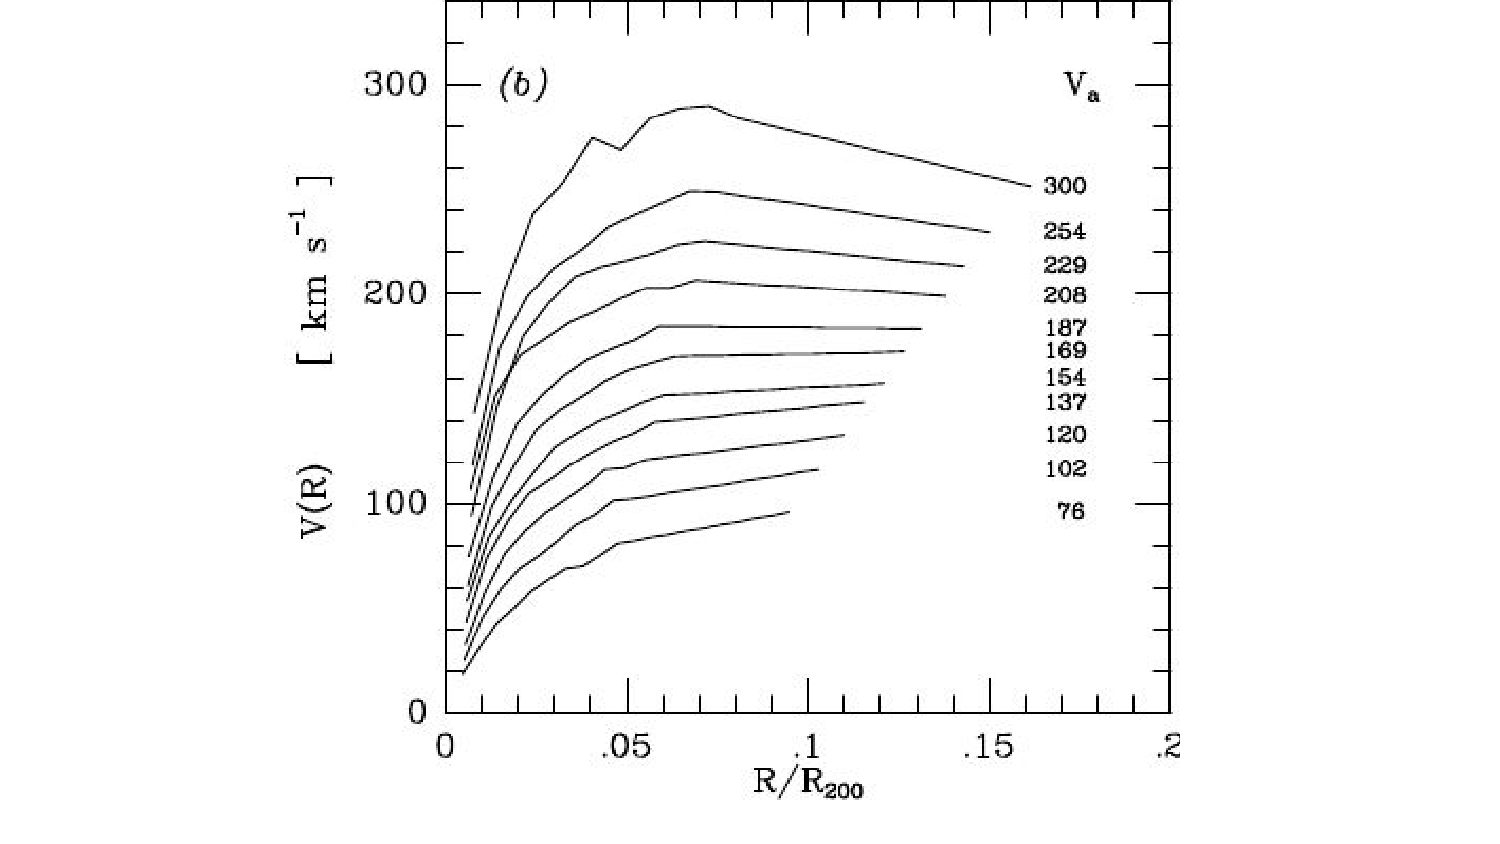
\includegraphics[width=\linewidth]{URC}
     \caption{Universal Rotation Curve spectrum, Used with permission from Ref.\citep{salucci}}
     \label{fig:URC}
\end{figure}
 
\newpage

 
 The standard dark matter rotation curve formula is

 \begin{equation}
v_{obs}^2 (r)=  v^2_{lum}(r) +  v^2_{dm}(r).  
\label{eq:zonte1}
\end{equation} 



Velocities  $v_{obs}$ come  from   
measurements of  Doppler shifted spectra $\omega'$      interpreted  by  Lorentz   Doppler shift formula 
 
 \begin{equation}
 \frac{v_{obs}}{c}=
\frac{  (\left \frac{\omega'(r)}{\omega_o}\right)^2 -  (\left\frac{\omega_o}{\omega'(r)} \right)^2 }{  (\left\frac{\omega'(r)}{\omega_o}\right)^2  +  (\left\frac{\omega_o}{\omega'(r)}\right)^2 } , 
\label{eq:modelLumA}
\end{equation} 

as relative frame motions. 


Velocities  $v_{lum}$ in Eq.~\ref{eq:zonte1} come from observations of total light in specific wavelengths which trace mass, and then yield  a mass-to-light ratio from Population Synthesis Models (CITE),
 
  \begin{equation}
v_{lum}^2 = \gamma_b v_{bulge}^2 +  \gamma_d v_{disk}^2 + v_{gas}^2,  
\label{eq:zonte3}
\end{equation} 
 
for the  $\gamma_i$  the  mass-to-light ratios of the stellar disk and bulge, and each mass contibution (disk, bulge and gas) again taken summed quadratically to represent a sum of masses by Poisson's equation.  





 

  Note,  population synthesis modeling  is an under-constrained field  precisely because the measurement of Doppler shifted spectra did not constrain $v_{lum}$, but rather introduced    an   new quantity of gravitating mass. 
 
  


then yielding orbital velocities by   Poisson's equation Eq.~\ref{whatsgood}.



Velocities $v_{dm}$ in Eq.~\ref{eq:zonte1} are attributed to    dark matter, and Eq.~\ref{eq:zonte1}  can be seen to be a quadratic mass sum  $M_{dyn} = M_{lum} + M_{dm}$   by Eq.~\ref{zoochance1}.
 


We modify the rotation curve formula in  Eq.~\ref{eq:zonte1} by  replacing dark matter  with  a series of two  Lorentz-type transformations and a curvature ratio,
   

\begin{equation}
v_{rc}^2 =  v_{lum}^2+\alpha \kappa^2 v_{1} v_{2} , 
\label{eq:zonteLCM}
\end{equation}  

 where all terms   are a function of $r$ except the model's free fitting parameter $\alpha$, which is single valued for each galaxy  fitted. 
 
 All terms $\kappa, v_1, v2$ are relationships between 
  the galaxy sending the signals  and that receiving them (MW). This is akin to field frame treatment (CITE Bertschinger).  Fitting details and analysis are reported in Sec.~\ref{sec:analysis}. 

 Terms in $\kappa$ 
are 
curvature ratios of the Newtonian gravitational potentials  

 \begin{equation}
\kappa=\frac{\Phi_{gal}}{\Phi_{mw}}  
\label{eq:kappa2}  
\end{equation}  
 
where the parametrization of the potentials is discussed in detail in Sec.~\ref{sec:gravDets}.
 

Terms in $v_1$ and $v_2$   employ a new technique of using Lorentz maps between slightly curved gravitational frames, foliated in Schwarzschild metric terms $g_{tt}(r)$. To construct these maps we note that 
  Eq.~\ref{eq:modelLumA}   is applicable to boosts between   inertial frames in a flat spacetime background.   Such a flat Lorentz transformation   can be  as in   written as a hyperbolic rotation  
  
     \begin{equation}
         \frac{v}{c} = \tanh \zeta = \frac{e^\zeta - e^{-\zeta}}{e^\zeta + e^{-\zeta}}   
         \label{boost}
     \end{equation} 

 for $\zeta$ a rapidity hyperbolic angle  relating two frames by  a rotation in Minkowski spacetime. We identify the 
    Lorentz exponential term  $e^\zeta = \omega'(r) /\omega_o$ as the frame-field term  and extend to the case of slightly curved field-frames (CITE RINDLER or MTW) . 
    
     
Terms in $v_1$   serve to   map between the two curved galaxy manifolds, 
 
   \begin{equation}
       v_1 = \sinh \gamma_c
   \end{equation}
 
 one-to-one in $r$. 
 The argument of the hyperbolic sine, $\gamma_1$ is identified with the Lorentz exponential, 
 
     \begin{equation}
     e^{\gamma_c}=  \frac{\omega_{MW}}{\omega_{gal}}  =\sqrt{\frac{g_{tt}|_{gal}}{g_{tt}|_{MW}}}  
      \label{eq:gravRS}
    \end{equation}
    
in the  weak field Schwarzschild  limit, where gravitational  redshift terms $g_{tt}$ are evaluated at the same $r$ in   two distinct galaxy manifolds (see Eq.~\ref{clocktime}). Discussion of this technique are given in Sec.~\ref{sec:gravDets}. 
  
The  second term, $v_2$  serves to map from the curved 2-frame Eq.~\ref{eq:gravRS} back  to the flat 2-frame where one makes observations.  That this second step is necessary is supported by the constancy of the speed of light,

\begin{equation}
\frac{v_{2} }{c}=  \cosh \gamma_2.
\label{eq:hyperbolico}
\end{equation}

The best $v_2$   Lorentz exponential term  is identified as
 
\begin{equation}
    e^{\xi}=   e^{(\gamma_c+\gamma_f)/2}.
\end{equation}

composed of the map of the curved 2-frame term $e^{\gamma_c}$ and the flat frame term $e_{\gamma_f}$ . 

 
 We identify the flat-frames with the frequency shifts expected from the Keplerian velocity profile $v_{lum}$, 

 \begin{equation}
     v_{lum} = \frac{\omega_l^2 - \omega_o^2}{\omega_l^2 + \omega_o^2}
 \end{equation}
 
for which  the Lorentz exponential term is 

\begin{equation}
    e^{\gamma_f}=\omega_{l}/\omega_o.  
    \label{eq:flat}
\end{equation} 
  
 

  
  
\subsection{gravity details \label{sec:gravDets}}


    W. Rindler's states  that ``the center of each galaxy provides a basic local standard of nonacceleration ... so then can be treated like a local inertial frame relative to our own center.''\cite{rindler2013essential}. We  use this idea to construct an extension from the standard gravitational redshift formula 
   
   \begin{equation}
       \frac{\omega_1}{\omega_2}  =\sqrt{\frac{g_{tt}|_{P2}}{g_{tt}|_{P1}}} =\sqrt{\frac{|\xi^t\xi_{t}|_{P2}}{|\xi^t\xi_{t}|_{P1}}}. 
      \label{eq:grav}
    \end{equation}
    
    
    which relates two points on a single gravitational manifold,  to   a frame relationship between two such distinct manifolds, by the time isometry of the Killing vector field 
   $\xi^t$.
    
    Key to 
our approach is   Rindler's observation  that it is the centers of each galaxy which can be compared inertially. 
 The ratio of frequencies in Eq.~\ref{eq:grav}   identifies the frame fields with the Schwarzschild time metric coefficients 


  \begin{equation}
      g_{tt}= -( 1 - 2\Phi/ c^2).
      \label{clocktime}
  \end{equation} 
 
  
 given here in the weak field    limit,  in Boyer-Lindquist coordinates \cite{Hartle}, \cite{Wald}, for $\Phi $
 the Newtonian  gravitational potential, and $c$ is the vacuum light speed.  


On inspection, then, to synchronize galaxy centers is to synchronize the clock terms   in $g_{tt}$.   If we  assume  all galaxies rotate around central black holes, then event horizons all galaxies define zero   coordinate clock time. The vanishing size of central black holes compared to  the stellar bulge, disk and gas halo means that this assumption places us essentially at $r\approx 0$. 
Since terms in $g_{tt}$ are really terms in  $\Phi (r)$, we  will synchronize clock terms by modifying the direction of the standard integration of  the Newtonian gravitational potential.    
   We integrate all gravitational potentials for this technique from the small $r$ limit as close to the event horizon as is possible, out  to the large $r$  extent of the data  

 \begin{equation}
      \Phi  = \left| \int^{R-big}_{r-small} \vec{F_r}\cdot\vec{dr} \right|.
      \label{eq:Newt2}
      \end{equation}
 
     Newtonian potentials integrated in this way  can then be compared from the same standard of rest. 
     Potentials calculated in this was still obey the central force law for test particles moving in circular orbits

\begin{equation}
 \frac{\partial \Phi_{lum}(r)}{\partial r}    =\frac{v_{lum}(r)^2}{r},  
    \label{zoochance1}
\end{equation}

 and Poisson's equation
 
\begin{equation}
\nabla^2 \Phi_{lum} (r) = 4\pi G \rho (r).   
    \label{whatsgood}
\end{equation}

 %line249 needs Poisson 



  The standard direction of integrating Newtonian gravitational potentials $\Phi$  is usually from the outside, the large $r$ limit, to the inside. The potential is then  assumed to be   zero at the large $r$ limit. This is an implicit assumption of a 
  a flat  embedding spacetime.  It is unnecessary and we also do not know the external embedding environments of galaxies (Hubble flow, dark energy content, curvature of the universe, etc). 
  
Since what  we physically measure is differences in potential, the important thing is to relate all potentials to the same notion of zero. 
Which then means to integrate all 
   $\Phi$ from the  point  where all the clocks can be said to be synchronized (at $r\approx 0$).
   Abandoning the assumption that all galaxies sit in the same external flat background potential is supported by the complexity  of flowlines in large groups of galaxies shown in the  symmetries of
the Dipole-Repeller (CITE Pomerades). 
   
   
   All terms in $\Phi(r)$ used in this paper  are those  integrated from reported in the      SPARC  library(CITE LELLIE 2016) for  luminous velocities $v_{lum}$ as in Eq.~\ref{eq:zonte3}.  Assumptions in their reported luminous mass models and RCFM mass-to-light ratios are included in Sec.~\ref{sec:analysis}. 
 
 

 
  
    


\subsection{Geometry Isomorphism}
As noted by \citet{PhysRevD.70.083509}, in the parts of galaxies where rotation curves become flat the geometry of the enclosed mass is essentially spherically symmetric. 
In the plane of the galactic disk, the use of spherical geometries is isometric to an  exponential thin disk introduces  \citet{Chatterjee}. The spherical geometry of a sphere (vis. Schwarzschild) will overestimate the gravitational potential inside of $r< R/3$, and are essentially commensurate   for $r>R/3$. That said, outside of the length $R$ characterizing the stellar disk (Fig.~\ref{fig:my_geom}),  the   gravitational potentials for both follow the same line shape and Keplerian decline  ($\alpha = 1.0$). Therefore, use of the Schwarzschild geometry as proof of concept does not introduce any artifacts, aside from overestimaing the barynoic potential inside of $R/3$. 
 
 
\begin{figure*}
    \centering
    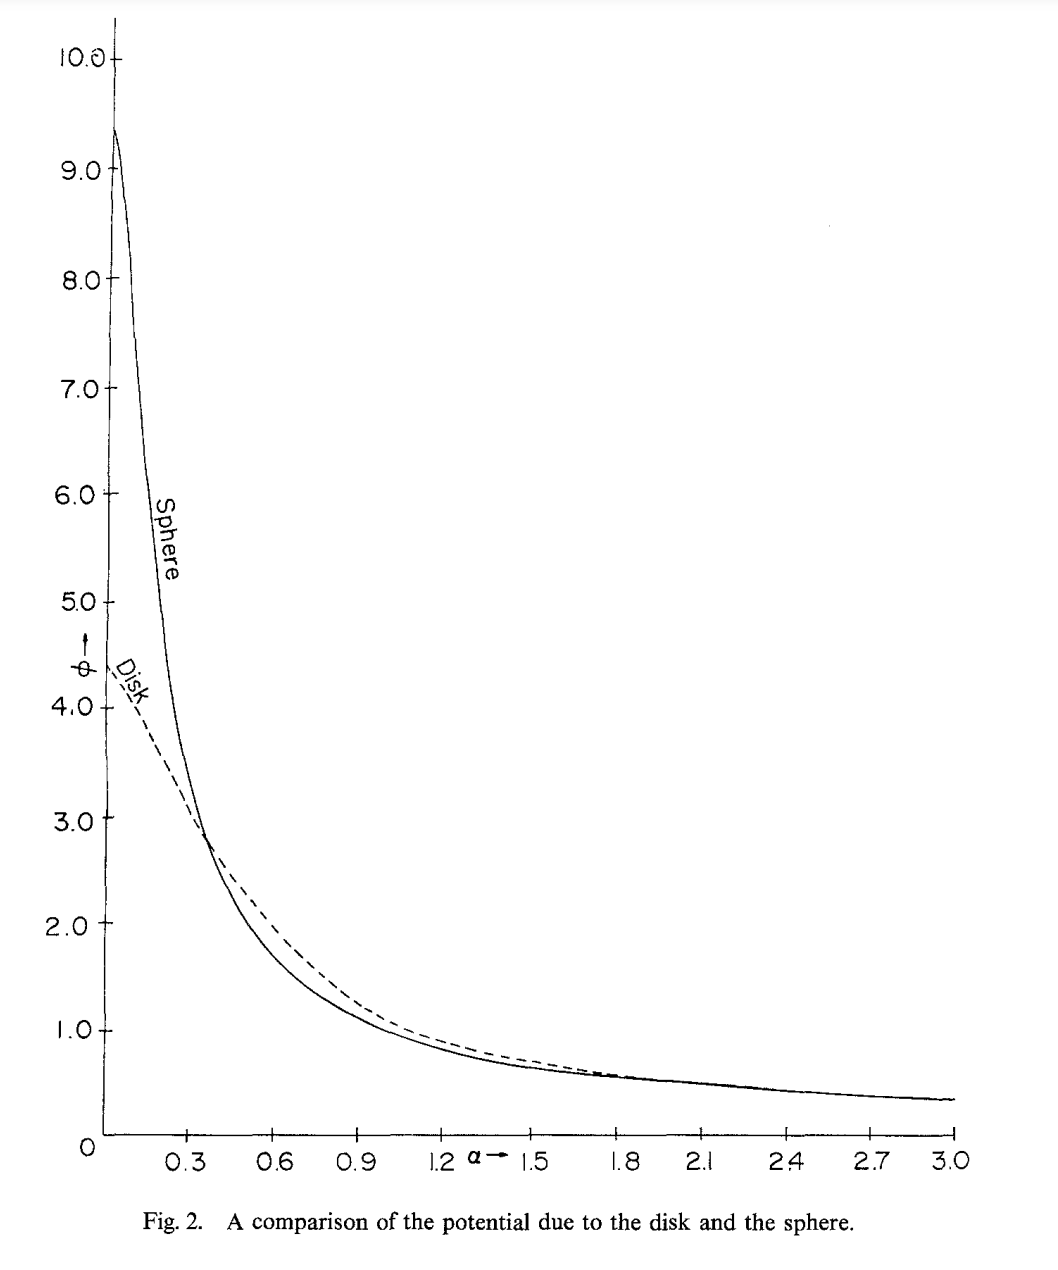
\includegraphics{Chatterjee_SphereDisk.png}
    \caption{A $\alpha = r/R$ for $R$ the radial extent of the stars \cite{Chatterjee}}
    \label{fig:my_geom}
\end{figure*}
  Results indicate that the potential due to the sphere and the disk along its plane are equal at a distance of about 1/3R, where R is the radius of either configuration. Interior to this distance, the potential due to the sphere is greater than that due to the disk and beyond this distance vice versa.
  
  
  
%%%%%%
%%%%%%%
%%%%%%
%%%%%%
\section{Analysis on  the SPARC data set\label{sec:analysis}}
 
The
 SPARC sample we test in this paper.  
 
\subsection{Luminous Mass modeling in the SPARC library}
as in Eq.~\ref{eq:zonte3}
 
In RCFM fits reported here, the    bulge and disk mass-to-light ratios are allowed to vary freely (See Eq.~\ref{eq:zonte3}), though the average values are within stated criteria   \cite{2016Lelli} of $\pm 20\%$. The gas fractions (HI scaled for Helium abundance) are fixed though addition of molecular gas could increase mass fractions in the inner kiloparsec of a galaxy(CITE RENE WB). 



 
 We fit the SPARC sample of Spitzer Photometry and Accurate Rotation Curves for 174 galaxies  \cite{2016Lelli} wiht the RCFM presented here. 
We compare results with the work from MOND and RAR spanning  \citet{McGaugh_2014}- \citet{Li_2018}. 
  
 
%%%%%%
%%%%%%%%
%%%%%%
%%%%%%%
%%%%%%
%%%%%%
\subsection{Milky Way}
{\color{red}justify choose Xue Sofue   MW in this paper. }

{\color{red} \rule{\linewidth}{0.5mm}}

 All terms in $ \kappa^2 v_{1}v_{2}$ require an assumption of the Milky Way  baryon profile which is notoriously underconstrained. We choose here to use 
 a hybrid model from \cite{Xue} and \cite{Sofue}. Other static MW profiles are available at the Git repo: Cisneros-Galaxy/RCFM. 

IN \cite{Li2016ModellingMD} the bulge is more like Sofue. Not flat like McGaugh. 
To understand why. 
``using the recently released Gaia billion-star map8
, we propose a
Galactic disk mass distribution model which is based on the star density distribution
rather than the brightness and mass-to-light ratio. ''
TROUBLE: ``we obtain a flat rotation curve
which reproduces the key observed features with no need for a dark halo''.


 
\subsection{Correlation to  the model's free parameter }
 
We transition the idea of excesses in Doppler shifted spectra from a  pure kinematic interpretation, in which terms in  $v_{obs}$ above estimates for  $v_{lum}$ represent real, orbital motions, to a regime in which the excesses in $\omega'$ represent.
  relative gravitational redshifts between the extended gravitational  frames of  galaxies. 
 The baryonic mass models reported in any rotation curve study are only as good as    as the distance estimate, so to train the model's free parameter we select a subset of galaxies who have Cepheid or Tip of the Red Giant Branch distance measurements.  When the free parameter is fixed to a constant value, we will then run on the entire SPARC data set, with the exception of 20-30 galaxies where Lelli et all 2016 excluded those galaxies which have an inclination greater than $85^o$ as impossible to constrain a proper surface brightness profile, and those at inclinations less than $35^o$ as being impossible to accurately report line of sight Doppler shifts.   
 We   explore the    model's free parameter space using a subset of the SPARC galaxies, selected based on  the most reliable distance estimates,   Cepheids and Tip of the Red Giant Branch (CITE McGaugh).   By this criteria, we select 46 galaxies, plotting the free parameter for each galaxy versus the ratio of the total luminosity $L_{total}$ to    the half-light radius $R_{eff}$ \cite{Lelli_2016surface},  
 
 \begin{equation}
     \rho = L_{total}/R_{eff}
 \end{equation}
 
  which we find to be   strongly correlated to   $\alpha$. 
  
 \begin{figure*}[h]
\scalebox{0.5}%
{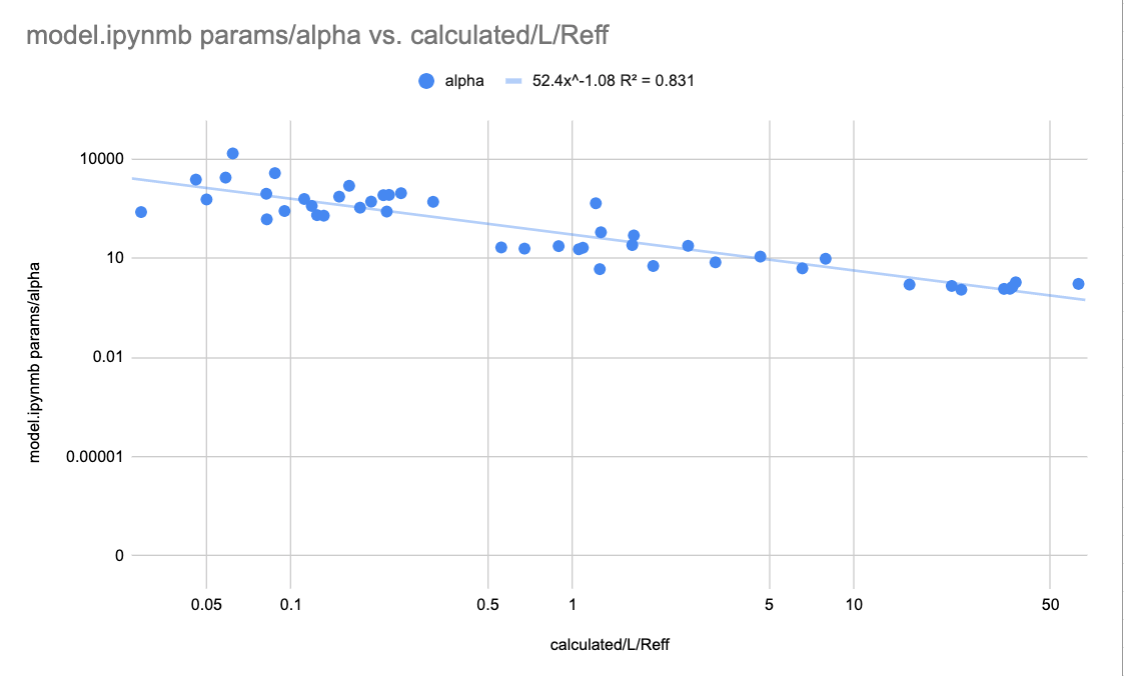
\includegraphics{alpha_10_18_22.png} }
\caption{ Remake this graph, nice like }
\label{alpha2}
\end{figure*}  
 
for 
\begin{equation}
    \alpha = 
\end{equation}



We might assume that $\alpha$ is a ratio of the same quantity for  the Milky Way $\rho_{mw}$ with respect to the other   galaxy $\rho_{gal}$  

\begin{equation}
\alpha=\left(\frac{\rho_{mw}}{\rho_{gal}}\right)^{b}  ,
\label{correl}
\end{equation}

then we arrive at a similar fit (See Fig.~\ref{alpha1}.



 

  
 
\section{MOND Comparisons}


While error    estimates have not been standardized across the field~\citep{Blok,Gent,Toky},     one can reliably   compare fits to the same data with the same reported errors. The     reduced $\chi^2_r$ values printed on each graph, but goodness of fit can also be visually appraised.  
 
 In MOND,  classical gravity is transitioned to  a paradigm where the luminous mass is the only mass  but    the acceleration scale of gravity changes on the enormous distance scales of galaxies.  As a heuristic  relativistic extension of MOND,  
  considering relative curvatures with respect to the Milky Way, we repeat MOND's successes and (MEAGAN and RICH) are 3 times more efficient at fitting the same rotation curves. 
 
% \cite{McGaugh2016RAR} is the other one. This one describes the sample. 175 SPARC galaxies. Describes all the assumptions for the disk, gas, bulge models, the band used and reasoning, rotation curve data from HI, 
 
% They only fit a subset (153 of 175) of these galaxies.I get 128, I guess I'm cutting endpoints of 85 and 30 and they include. Plus I exclude like five that I think fail to fit
 
  

 
  
 \section{  Conclusions   }
********
******
 
{\color{red} This heuristic replacement of dark matter is not fundamental in nature, but    one supposes if it is possible to quantify these
excesses in shifted spectra using entirely luminous mass as we do in this paper,  then a   fundamental derivation may exist.  The curious conspiracy of the luminous mass to   determine the dark matter  is here rephrased as a question of imprints from our Milky Way on Doppler shifted spectra.  This model has a static choice of the Milky Way, which is under-determined, as well as a free parameter.  
 }
 
 

  
 
%Places where dark matter is invoked. Structure formation: put spherical model replace flat, solve. Galaxy clusters, same,put flow lines on surfaces supported by dark energy. Tully Fisher: temp dependence with mass - but read Beckenstein's description carefully. Hemakes some points.  
   
However, both MOND and dark matter theories interpret the observed Doppler shifted spectra as physical velocities, and both modify classical physics \cite{de_Blok_2010}.   
We   present here a new picture of flat-rotation curves which does not   modify physics, but adds a new tool to the standard transformations of   relativity. 
What is presented is not a fundamental derivation of such transformations, but only a heuristic model   of spiral galaxies. 
We do not interpret excesses in Doppler shifted spectra as physical velocities, but rather as due to the Milky Way frame's imprint on the galaxy spectra we are receiving. 
 
 
 The second important building block of the new rotation curve interpretation  presented here   is from      the Universal Rotation Curve (URC) discovered by   Persic and Salucci and Rubin \cite{salucci}, \cite{Persic},  \cite{1978Rubin}.  The URC is  a collection of  1,100 galaxy rotation curves   plotted on the same   axes  and normalized by the  respective galaxy scale-lengths.  As can be seen   in Fig.~\ref{fig:URC},    
 the spectrum   inflects about   the assumed rotation curve of our   Milky Way.  Interpreted through a dark matter lens, the URC requires  
   galaxies smaller than the Milky Way to be more successful at accretion of    dark matter halos, than those    larger than the Milky Way.
   This means,  smaller masses tend to be   proportionally more successful at assembly of  larger dark matter halos counter to    classical gravitation theory.    In the simpler RCFM perspective,  the URC spectrum    represents the frame dependence of our Milky Way imposed onto the spectra  we receive  from external galaxies.  
 
  

%%%%%%
%%%%%
%%%
%%
%
%%%%%%


 % \caption{Results   for SPARC Luminous mass profiles  [NOT UPDATED]\label{sumRESULTS}}
 % \begin{tabular}{@{}llccccccc@{}}
 % \hline
 %  Galaxy     	  &Ref.~&  \multicolumn{3}{c}{\underline{ Other Model Fit Results}}	& & \multicolumn{3}{c}{\underline{LCM Fit Results }}  \\
%\hline
%   	 	& & &  $M/L_{disk}$		& $\chi^2_r$	&&$M/L$&$r_e$&$\chi^2_r$ \\ 
% \hline
%F 563-1	& 2	%& 			
%					&NFW	&--	 		&-- & 	&1.13 	&2.84 	&0.06 \\
%M 31* 	& 12 	%&7.5
%					&ISO	 	 &7.50		&0.36 & 	&5.88	 &4.80 	&0.04  \\
%M 33		& 5	 %&	K 		
%					& NFW 	&0.70		&2.46&  	 &1.98	 &1.46	& 0.17 \\
%NGC 891*	& 11 	% &3.6$\,\umu$m 
		%			&MaxLight &0.9 			&1.10  & 	 &--  	 &	&0.25 \\ 
%NGC 925 	&3	%&3.6$\,\umu$m
 			%		&ISO 	&0.18		 &2.40& 	&0.92	 &4.35	&0.11 \\
%NGC 2403	 & 3	%& 3.6$\,\umu$m
		%			& NFW	&0.41 	 	&4.56& 	&1.12	 	&2.18		& 0.88 \\
%NGC 2841*  &6-3	% & 3.6$\,\umu$m
%					&  James	&0.74 	 	&0.45 & 	&6.25	  &4.84	&0.11 \\
%NGC 2903  &10	 %&B	   		
%					&MOND   	&3.60 	 	&10.71& 	 &2.2	 	&2.81		&0.47\\
% NGC 3198 & 3 	%&3.6$\,\umu$m
%					 &NFW	&0.80	   	&5.40  &   	 &1.80 	 &5.10	&0.64   \\
%NGC 3521  & 8-6	 %&3.6$\,\umu$m 
%					&MOND	&0.71 	 	&0.97 & 	 &2.13  &3.23	&0.22 \\
%NGC 3726	& 10	%&B 			
%					&MOND	&1.00	 	&3.57& 	&1.06	 &2.70	&0.05 \\
%NGC 3953	& 10	%&B 			
%					&MOND	&2.7		 	&1.35& 	&1.79 	&2.60 	&0.35 \\
%NGC 3992	& 10	%&B 			
%					&MOND	&4.93	 	&0.50& 	&2.45 	 &4.77	&0.04 \\
%NGC 4088	& 10	%&B 			
%					&MOND	&1.16		 	&1.70& 	&5.58	 &2.70	&0.27 \\
%NGC 4138	& 10	%&B 			
%					&MOND	&3.5		 	&2.12& 	&3.67	 &1.46	&0.01 \\
%NGC 5055*	 & 3	%&3.6$\,\umu$m 
%					&  NFW	&0.79	 	&17.23&  	&5.87	 &3.29	&0.69 \\
%NGC 5533*	 & 10 %&B 			
%					&MOND	&0.6		  	&1.57 & 	&7.11 	  &3.23	&0.22  \\
%NGC 5907*	& 10	%&B 			
				%	&MOND	&1.6 		 	 &0.44& 	&2.04	 &3.45	%&0.09 \\
%NGC 6946*	&  10	 %& B			
%					&  MOND	& 0.5		 	&   3.03& 	&1.44 	 &0.76	&0.07  \\ 
%NGC 6946*	&  3	 %& B			
%					&  NFW	& 0.5		 	&   3.03& 	&1.44 	 &0.76	&0.07  \\ 
%NGC 7331	&8	% & 3.6$\,\umu$m
%					&James	&0.4 		 	& 0.45& 	&1.34	 &2.44	&0.09 \\
%NGC 7793  &14	%&B			
%					&ISO		&2.6		 	&1.08& 	&2.7	 &1.51	&0.11 \\
%NGC 7814* &11 	% & 3.6$\,\umu$m
%					&ISO   	& 0.68  	 	& 0.25& 	 &-- 	   &	&0.20 \\ 
%UGC 128		&6	%&				
	%				&James	&			&	&	&1.58	  &10.3	%&0.20\\
%UGC 6973	& 10	%&B 			
%					&MOND	&2.7		 	&23.5 & 	&--  	& 	&0.06 \\
%UGC 7524	& 6	%&B 			
%					&James	&--		 	&-- & 	&2.10 	&3.32 	&0.06 \\
% 1.~\citet{Bege}, 2.~\citet{JNav}, 3.~\citet{Blok} , 4.~\citet{Maria}, 
%5.~\citet{Cor03}, 6.~\citet{James},   7.~\citet{Batt},   8.~\citet{Gent},   9.~\citet{Bot},   10.~\citet{SanMcGa},
 % 11.~\citet{Frat},   12.~\citet{Car},   13.~\citet{giraud2000universal},   14.~\citet{Dicaire}, %15.~\cite{Klypin}. \\
%    \end{minipage}
%\end{table*} 


   

  \section[]{Acknowledgments}
 This work is dedicated to Emmett Till. This paper was written with gratitude on the usual, and accustomed  territories
of the Coast Salish, Cheyenne, Arapaho and Ute Tribal Peoples.
  The authors would like to thank  V.\,P.\,  Nair,   R.\, Walterbos, S.\ McGaugh, A.\, Klypin, K. Bender, C. Beetle and     T.\, Boyer.   \\
  
 
%The   dark matter problem  is currently woven into most faces of our cosmology (weaklensing, galaxy rotation curves, early structure formation, galaxy and cluster interactions).   We posit that not all of these problems are actually the same physics problem.  We will address in this paper only the dark matter problem in spiral galaxies, the so-called flat-rotation curve problem discovered by \citet{1978Rubin,Bosma78}. We believe the ideas presented here are extensible to the problem of galaxy and cluster interactions, and perhaps weak lensing, but not to early structure formation, which we believe to be a different physics problem. 


 \begin{figure}[h]
\begin{subfigure}{.5\textwidth}
  \centering
  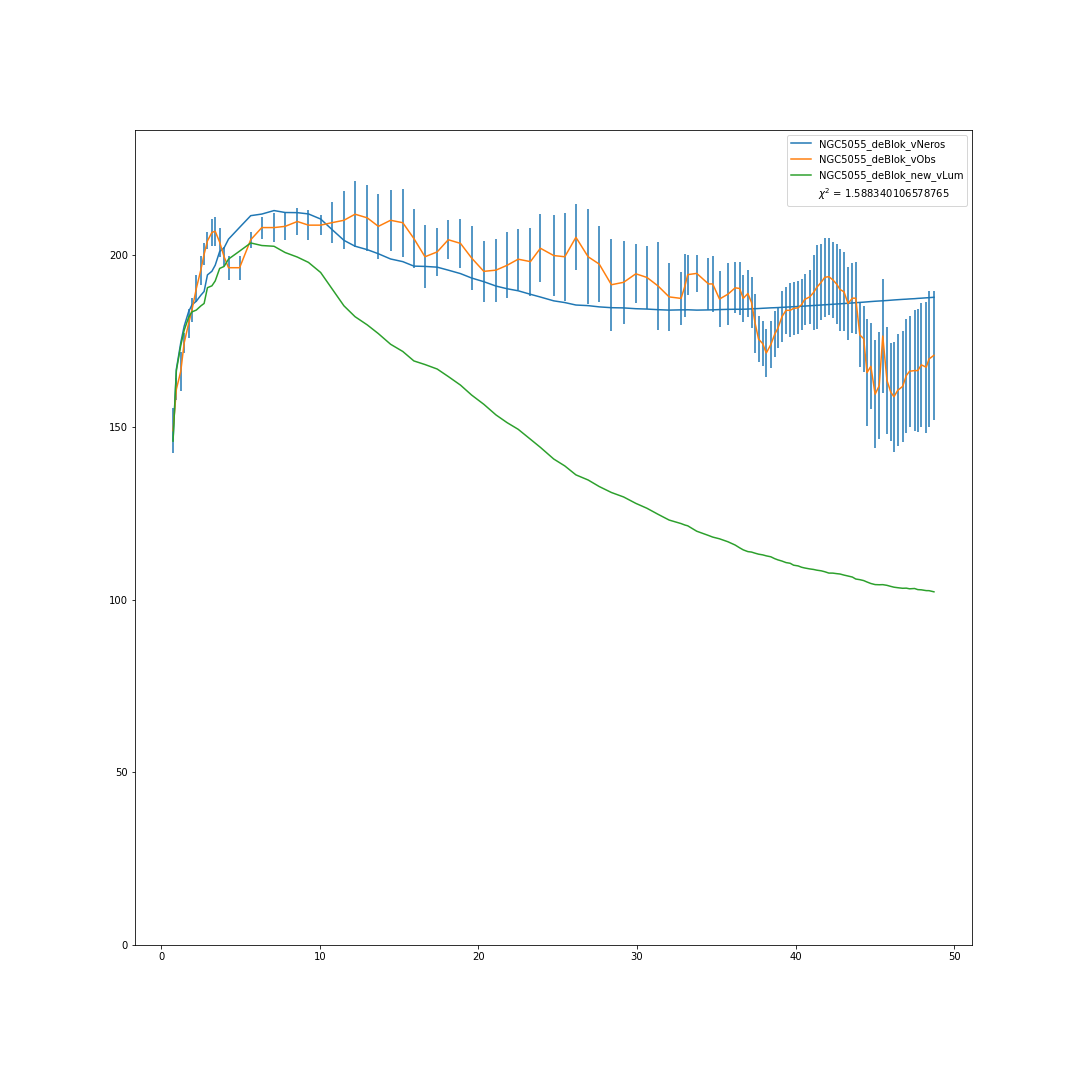
\includegraphics[width=.8\linewidth]{NGC5055_deBlok_XueSofue}
  \caption{deBlok\cite{Blok1}}
  \label{fig:sfig1}
\end{subfigure}%
\begin{subfigure}{.5\textwidth}
  \centering
  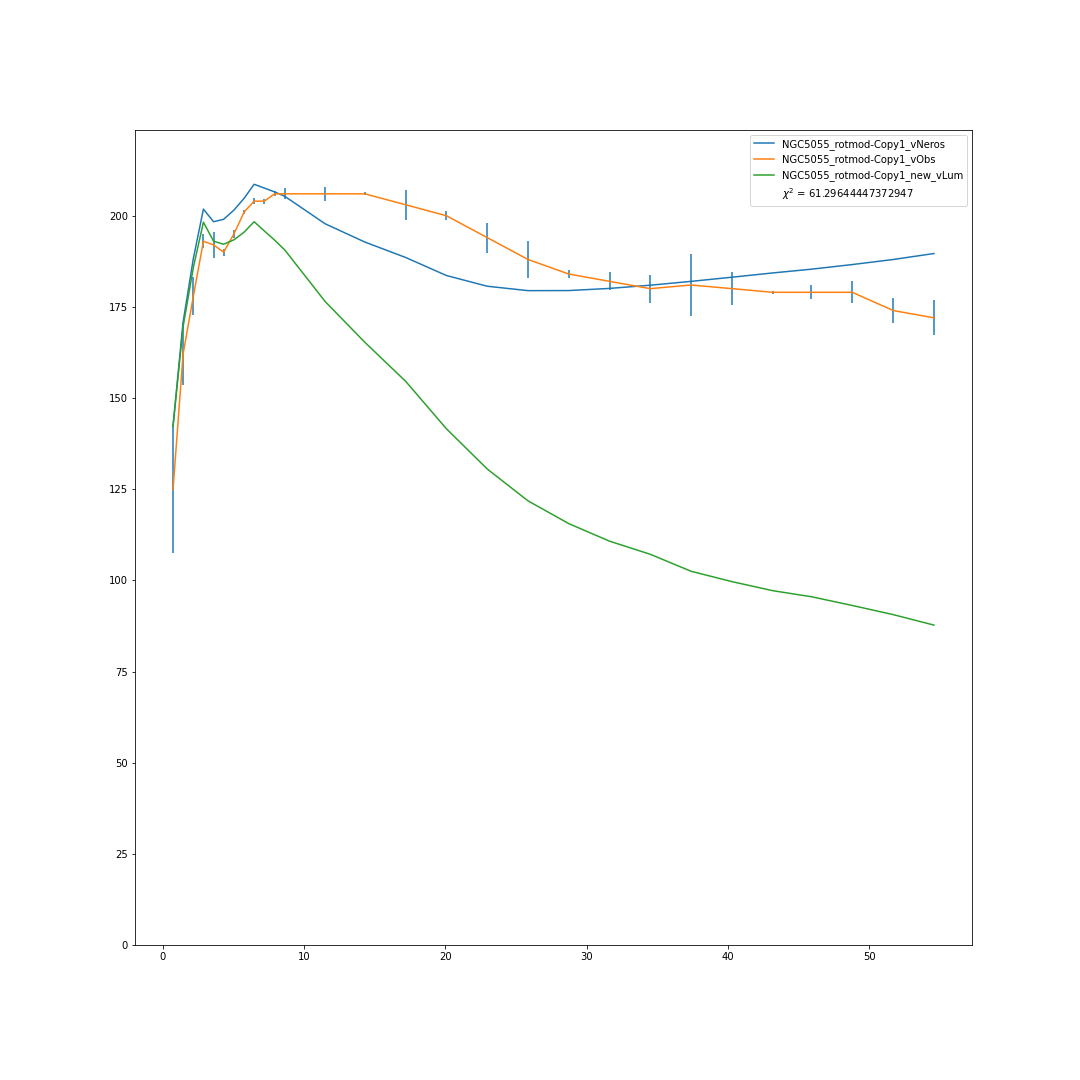
\includegraphics[width=.8\linewidth]{NGC5055_rotmod-Copy1_XueSofue}
  \caption{SPARC\cite{2016Lelli}}
  \label{fig:sfig2}
\end{subfigure}
\begin{subfigure}{.5\textwidth}
  \centering
  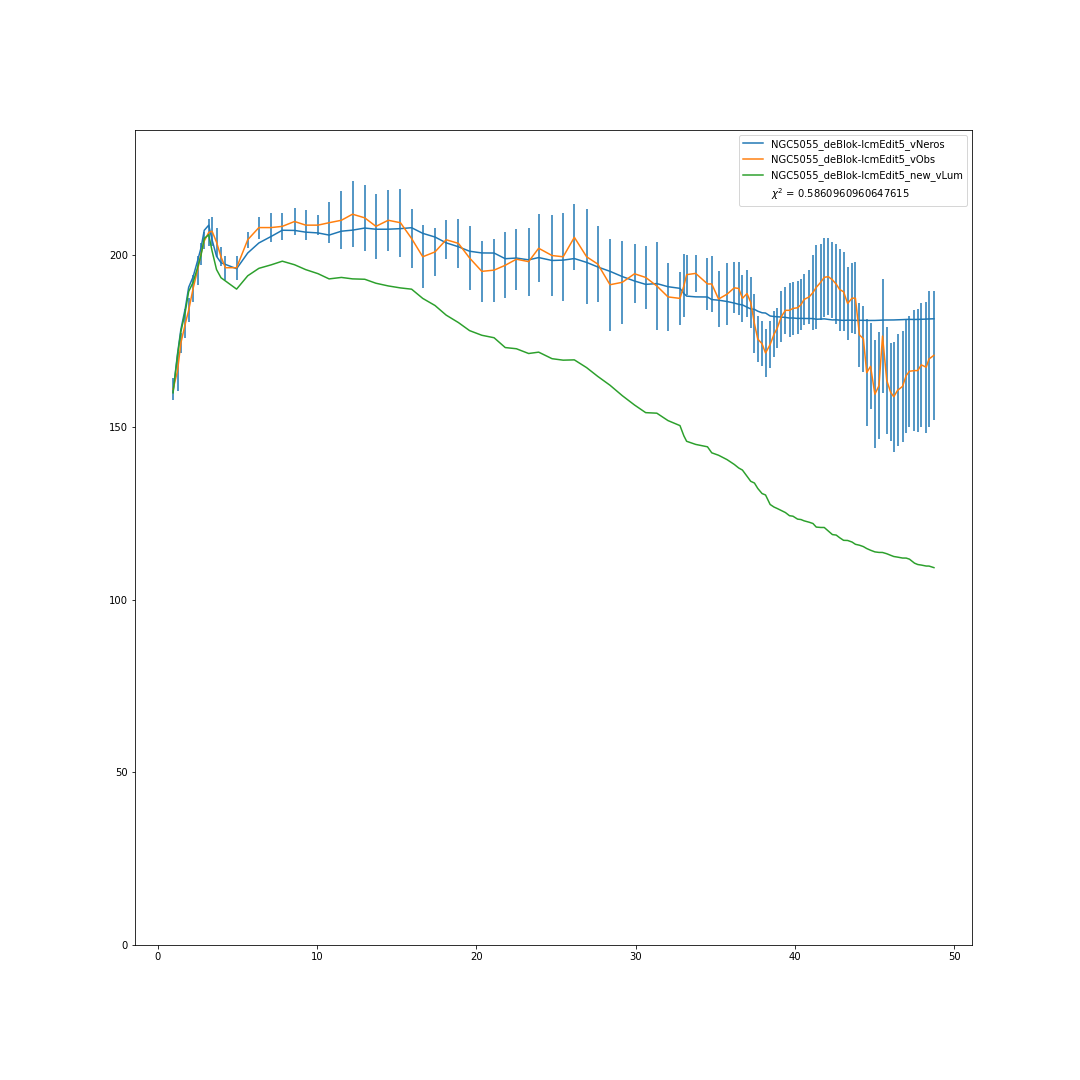
\includegraphics[width=.8\linewidth]{NGC5055_deBlok-lcmEdit5_XueSofue}
  \caption{Lum edits5 \cite{Blok1}}
  \label{fig:sfig3}
\end{subfigure}
\caption{RCFM fits of NGC 5055 }
\label{fig:fig5055}
\end{figure}
 
 
 
  \begin{figure}[h]
\begin{subfigure}{.5\textwidth}
  \centering
  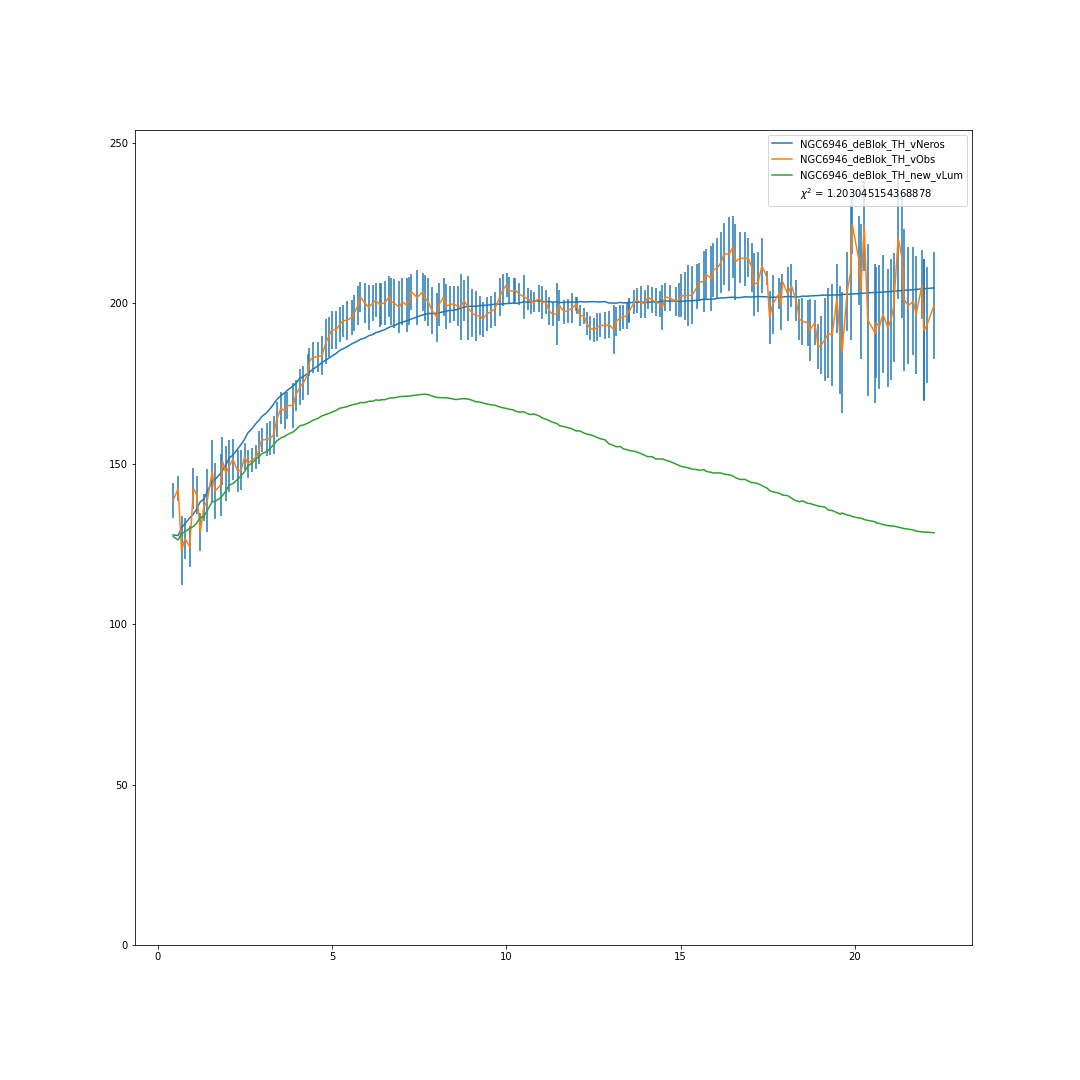
\includegraphics[width=.8\linewidth]{NGC6946_deBlok_TH_XueSofue}
  \caption{deBlok\cite{Blok1}}
  \label{fig:sfig4}
\end{subfigure}%
\begin{subfigure}{.5\textwidth}
  \centering
  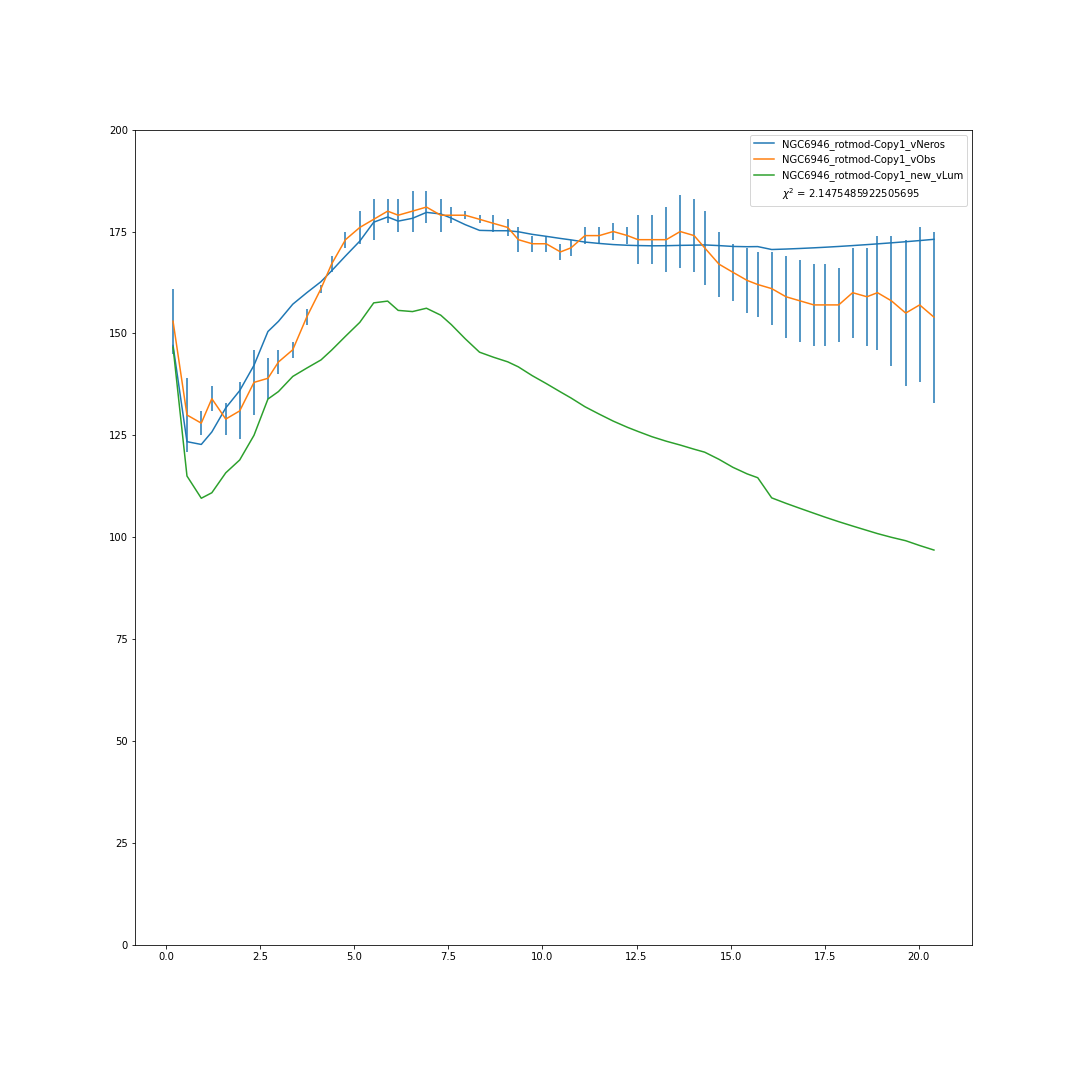
\includegraphics[width=.8\linewidth]{NGC6946_rotmod-Copy1_XueSofue}
  \caption{SPARC\cite{2016Lelli}}
  \label{fig:sfig5}
\end{subfigure}
\caption{RCFM fits  of NGC 6946 }
\label{fig:fig6946}
\end{figure}
%
%
%

  \begin{figure}[h]
\begin{subfigure}{.5\textwidth}
  \centering
  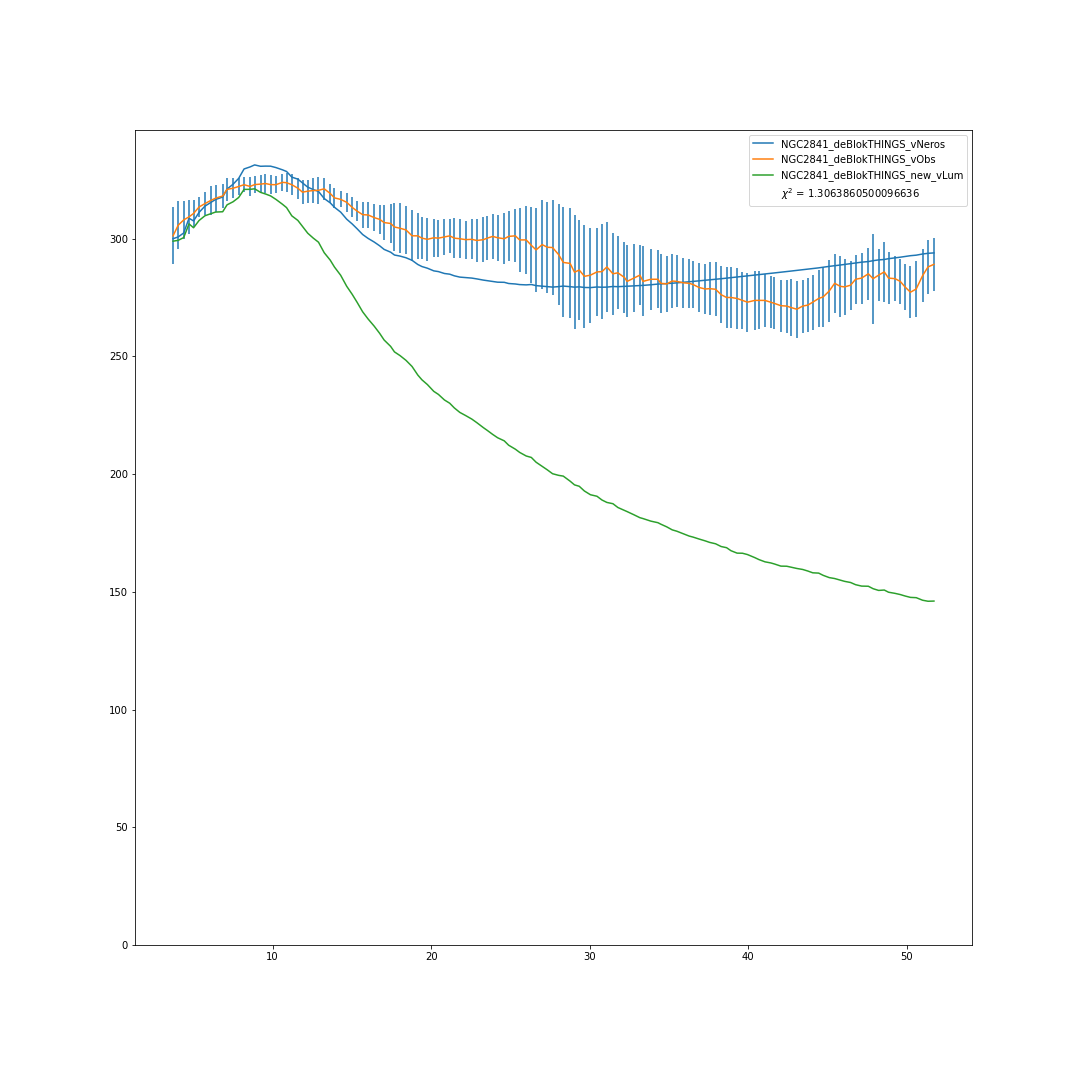
\includegraphics[width=.8\linewidth]{NGC2841_deBlokTHINGS_XueSofue}
  \caption{deBlok\cite{Blok1}}
  \label{fig:sfig9}
\end{subfigure}%
\begin{subfigure}{.5\textwidth}
  \centering
  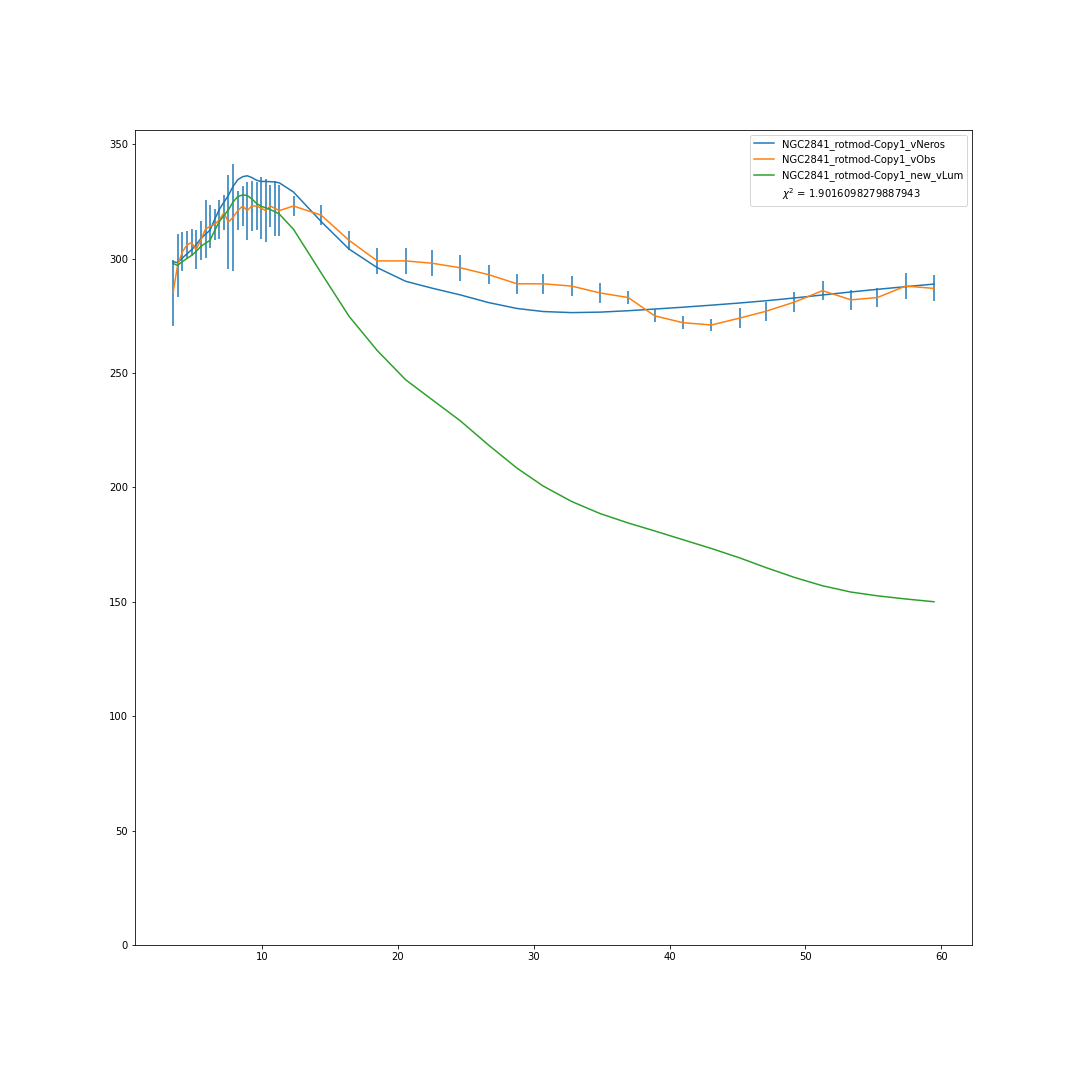
\includegraphics[width=.8\linewidth]{NGC2841_rotmod-Copy1_XueSofue}
  \caption{SPARC\cite{2016Lelli}}
  \label{fig:sfig10}
\end{subfigure}
\caption{RCFM fits  of NGC 2841}
\label{fig:fig2841}
\end{figure}

\clearpage
  \begin{figure}[h]
\begin{subfigure}{.5\textwidth}
  \centering
  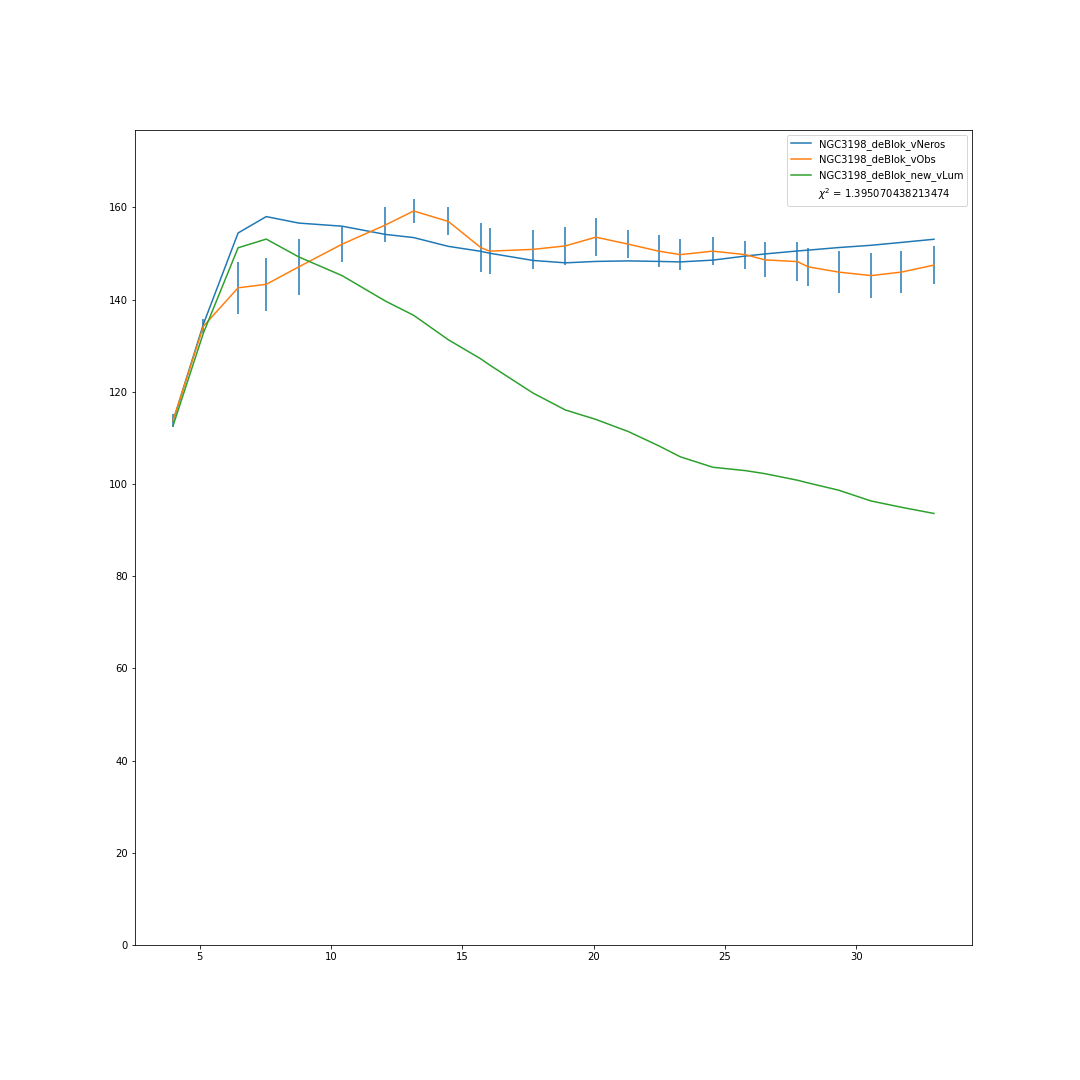
\includegraphics[width=.8\linewidth]{NGC3198_deBlok_XueSofue}
  \caption{deBlok \cite{Blok}}
  \label{fig:sfig6}
\end{subfigure}%
\begin{subfigure}{.5\textwidth}
  \centering
  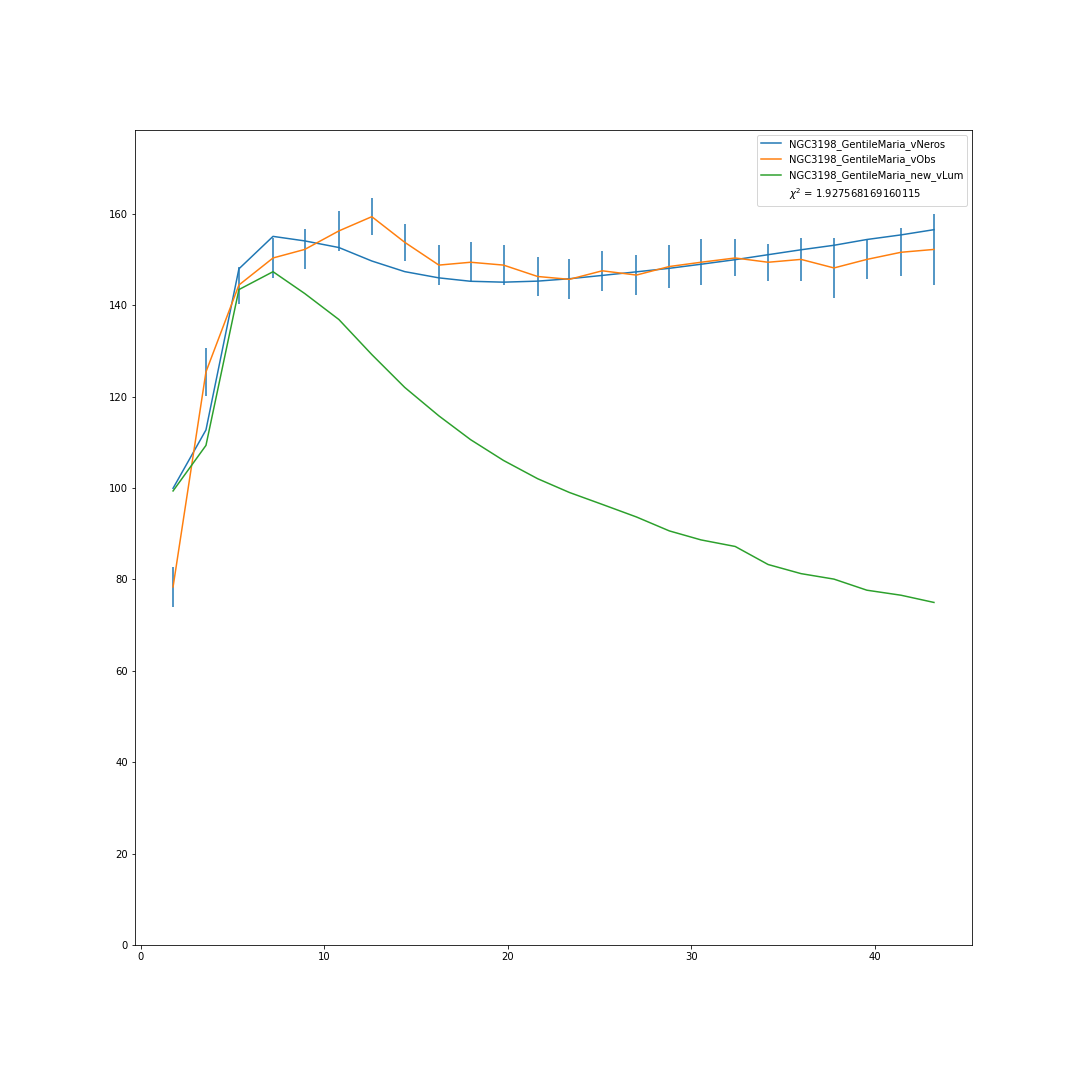
\includegraphics[width=.8\linewidth]{NGC3198_GentileMaria_XueSofue}
  \caption{Gentile \cite{Maria}}
  \label{fig:sfig7}
\end{subfigure}
\begin{subfigure}{.5\textwidth}
  \centering
  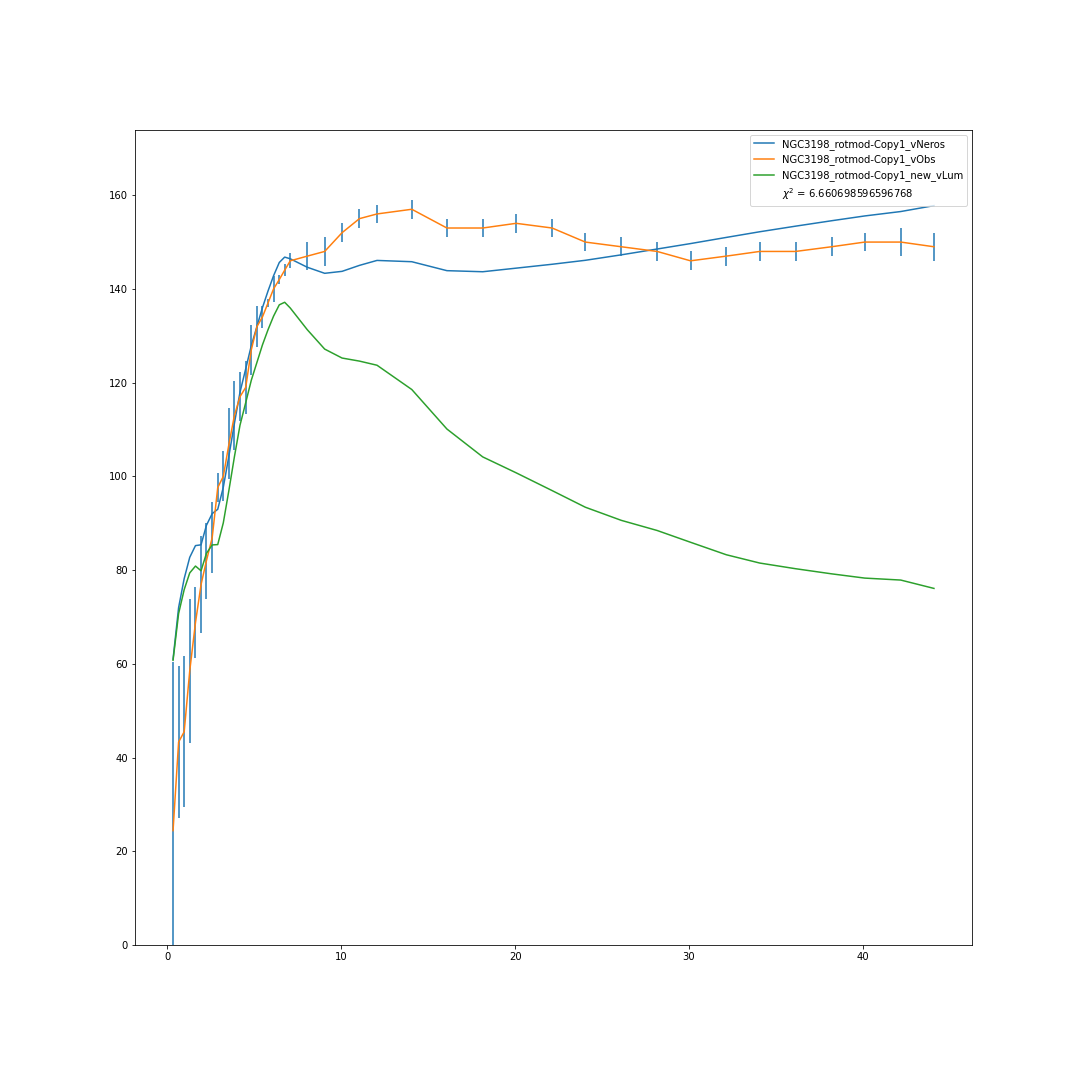
\includegraphics[width=.8\linewidth]{NGC3198_rotmod-Copy1_XueSofue}
  \caption{SPARC\cite{2016Lelli}}
  \label{fig:sfig8}
\end{subfigure}
\caption{RCFM fits  of NGC 3198}
\label{fig:fig3198}
\end{figure}
 %   
%
% 
\clearpage
%%%

  \begin{figure}[h]
\begin{subfigure}{.5\textwidth}
  \centering
  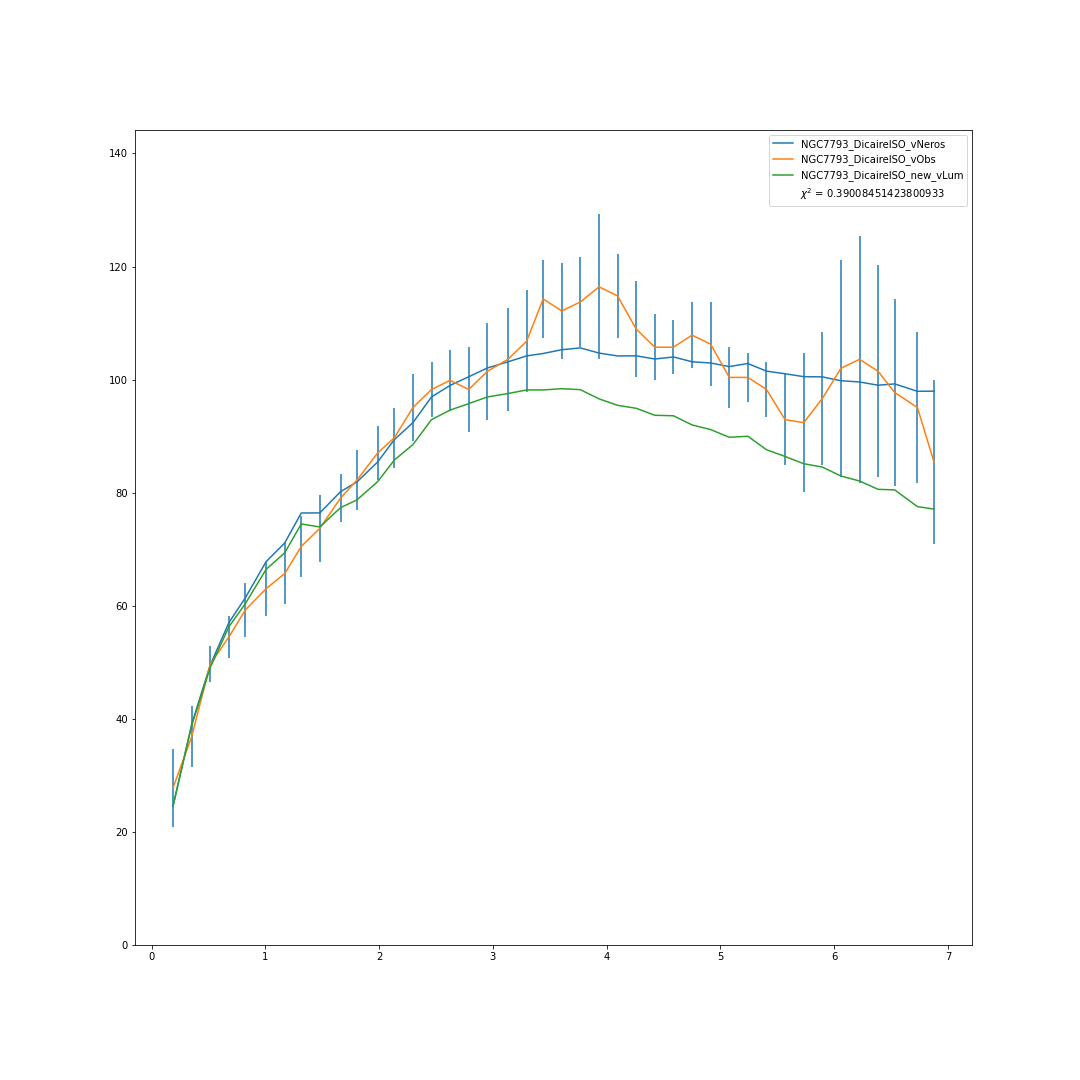
\includegraphics[width=.8\linewidth]{NGC7793_DicaireISO_XueSofue}
  \caption{Dicaire \cite{Dicaire1}}
  \label{fig:sfig11}
\end{subfigure}%
\begin{subfigure}{.5\textwidth}
  \centering
  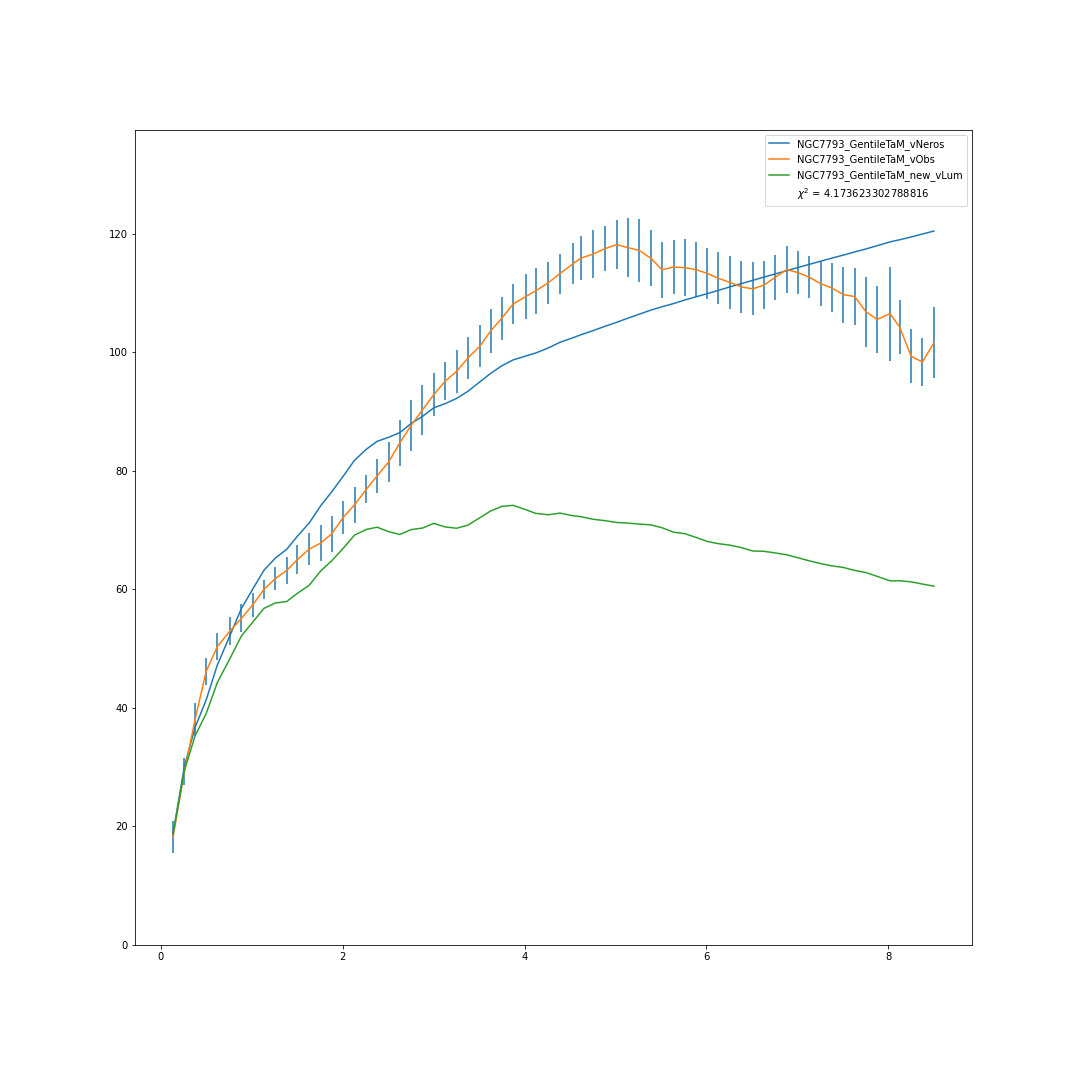
\includegraphics[width=.8\linewidth]{NGC7793_GentileTaM_XueSofue}
  \caption{Gentile\cite{Gent}}
  \label{fig:sfig12}
\end{subfigure}
\begin{subfigure}{.5\textwidth}
  \centering
  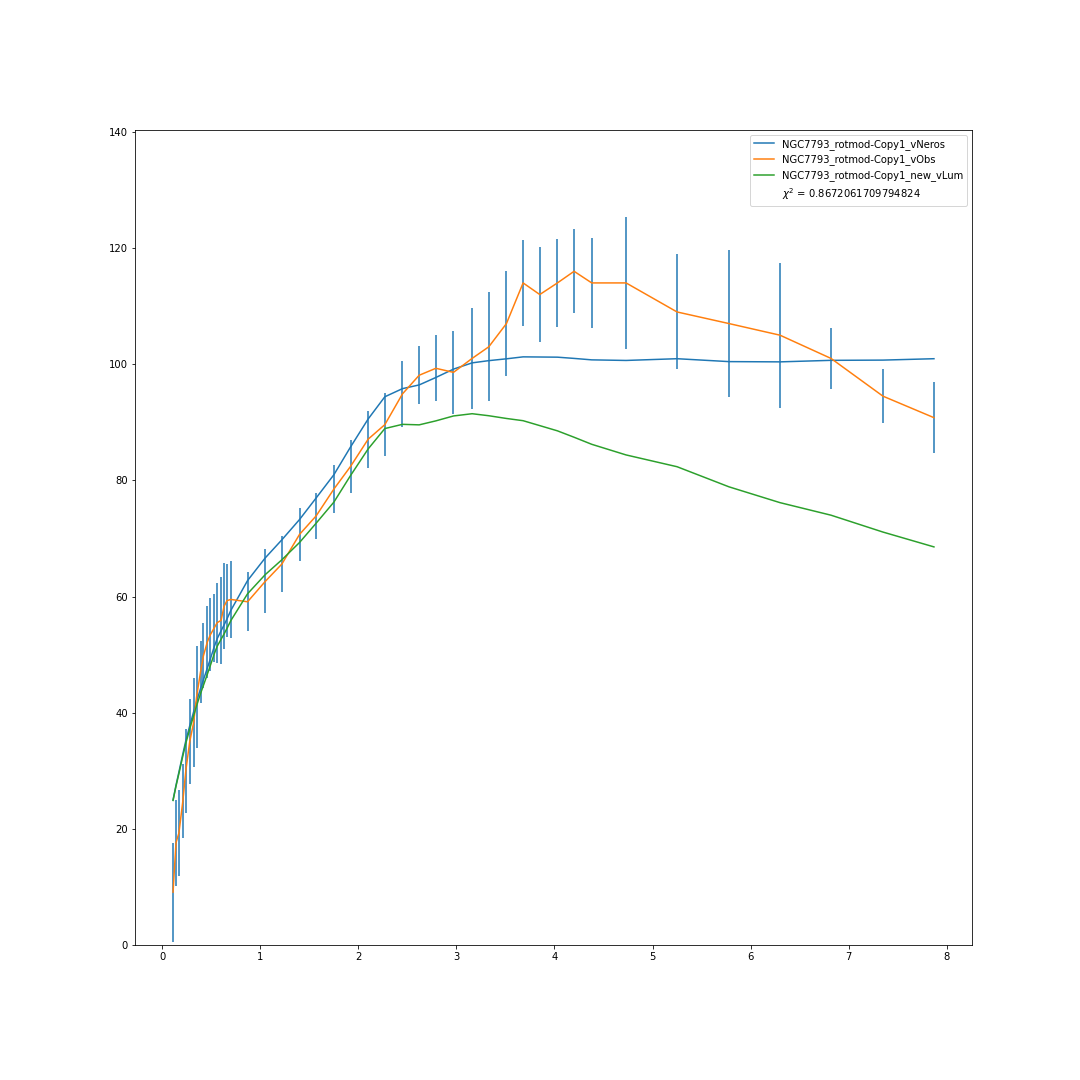
\includegraphics[width=.8\linewidth]{NGC7793_rotmod-Copy1_XueSofue}
  \caption{SPARC\cite{2016Lelli}}
  \label{fig:sfig13}
\end{subfigure}
\caption{RCFM fits  of NGC 7793}
\label{fig:fig7793}
\end{figure}
%
%
%
%
\clearpage
  \begin{figure}[h]
\begin{subfigure}{.5\textwidth}
  \centering
  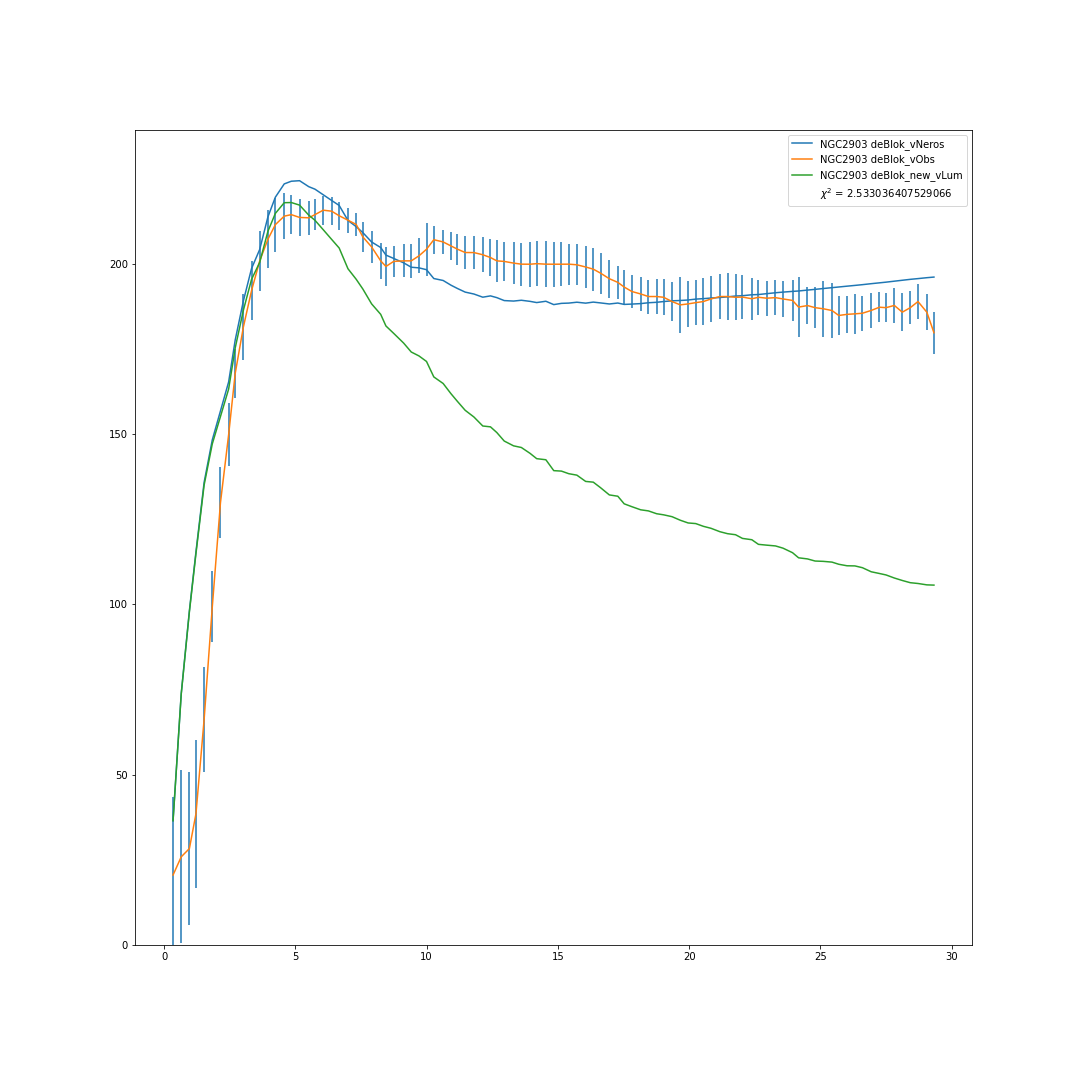
\includegraphics[width=.8\linewidth]{NGC2903deBlok_XueSofue.png}
  \caption{deBlok\cite{Blok1}}
  \label{fig:sfig14}
\end{subfigure}%
\begin{subfigure}{.5\textwidth}
  \centering
  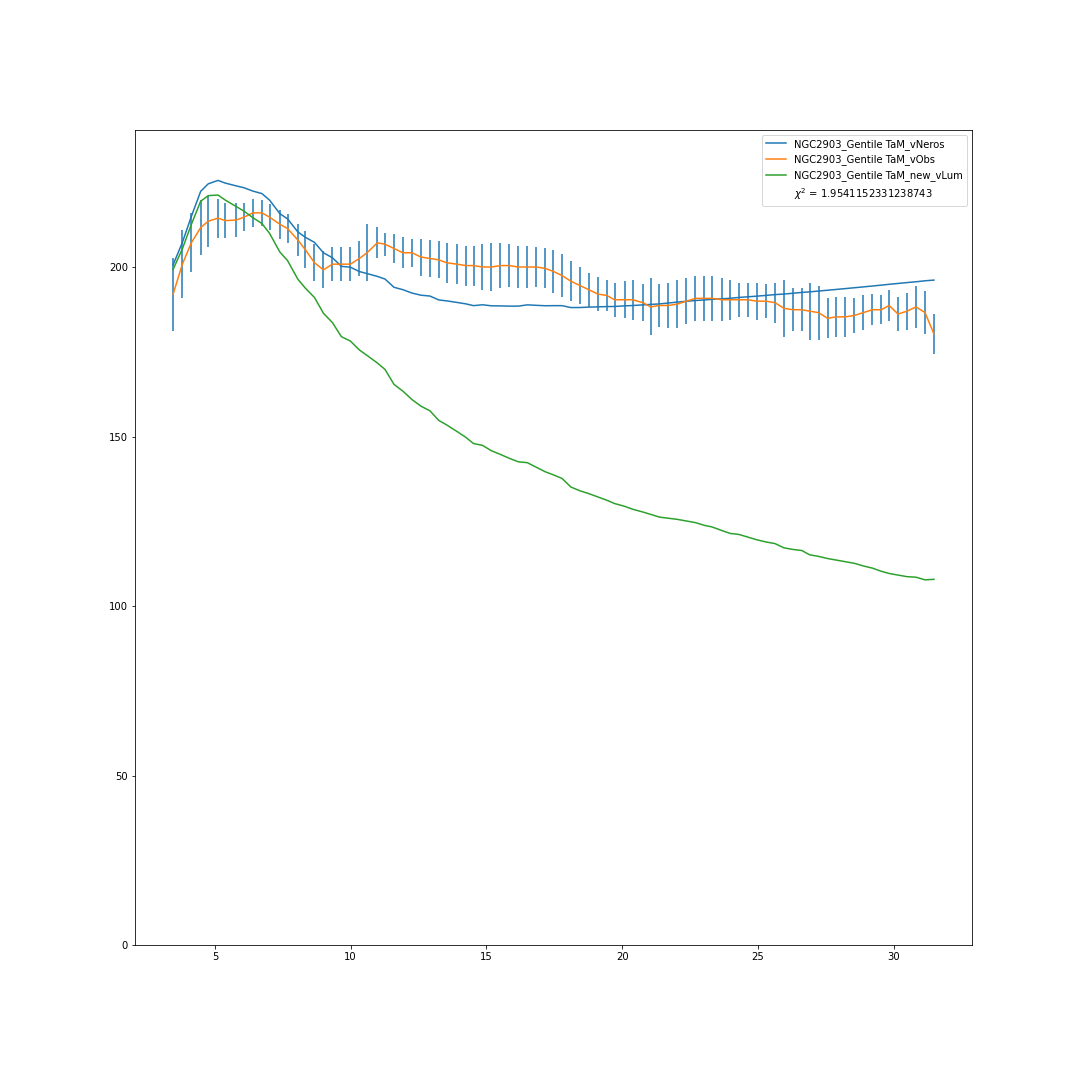
\includegraphics[width=.8\linewidth]{NGC2903_GentileTaM_XueSofue.png}
  \caption{Gentile\cite{Gent}}
  \label{fig:sfig15}
\end{subfigure}
\begin{subfigure}{.5\textwidth}
  \centering
  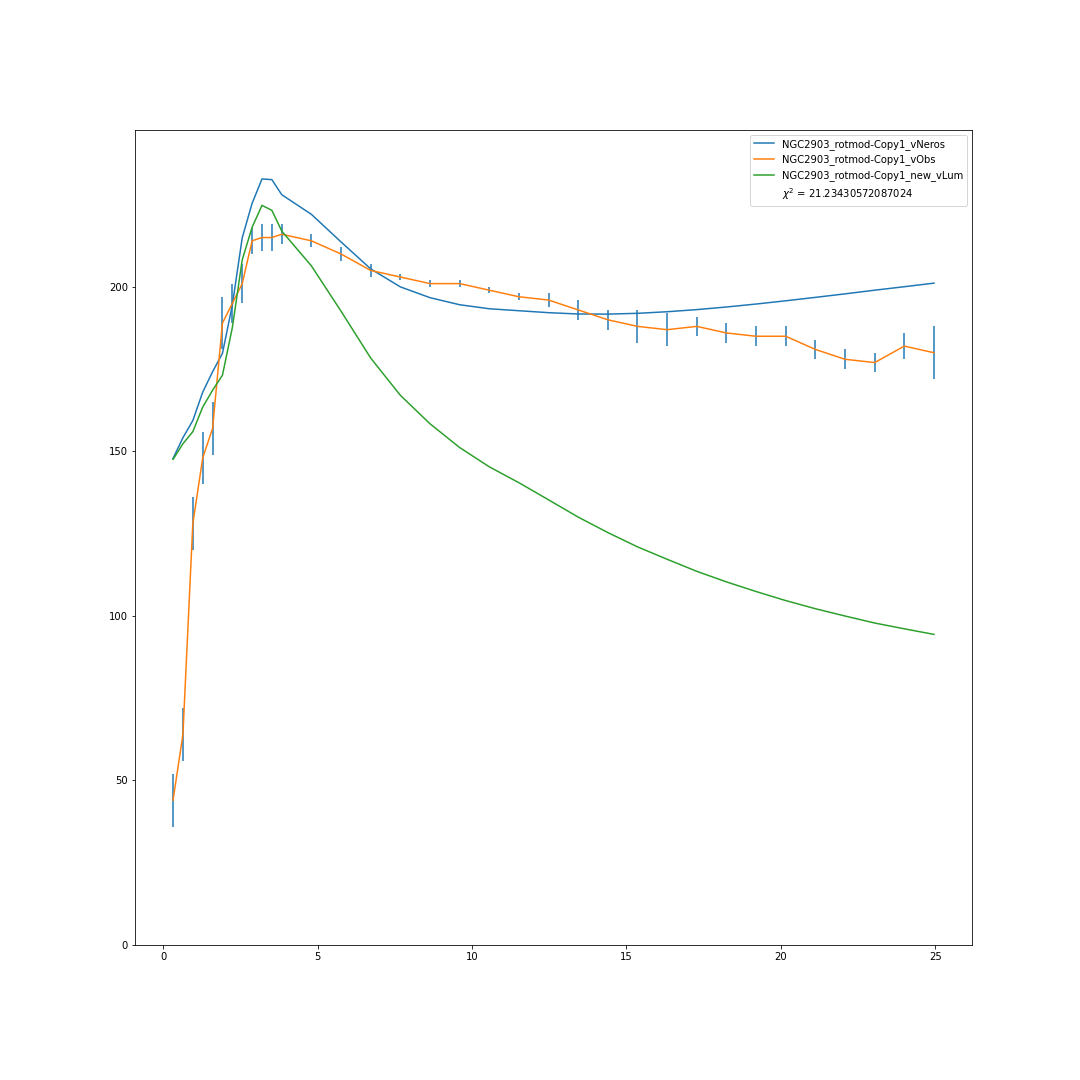
\includegraphics[width=.8\linewidth]{NGC2903_rotmod-Copy1_XueSofue.png}
  \caption{SPARC\cite{2016Lelli}}
  \label{fig:sfig16}
\end{subfigure}
\caption{plots of NGC 2903}
\label{fig:fig2903}
\end{figure}
%
\clearpage
%
%  
  \begin{figure}[h]
\begin{subfigure}{.5\textwidth}
  \centering
  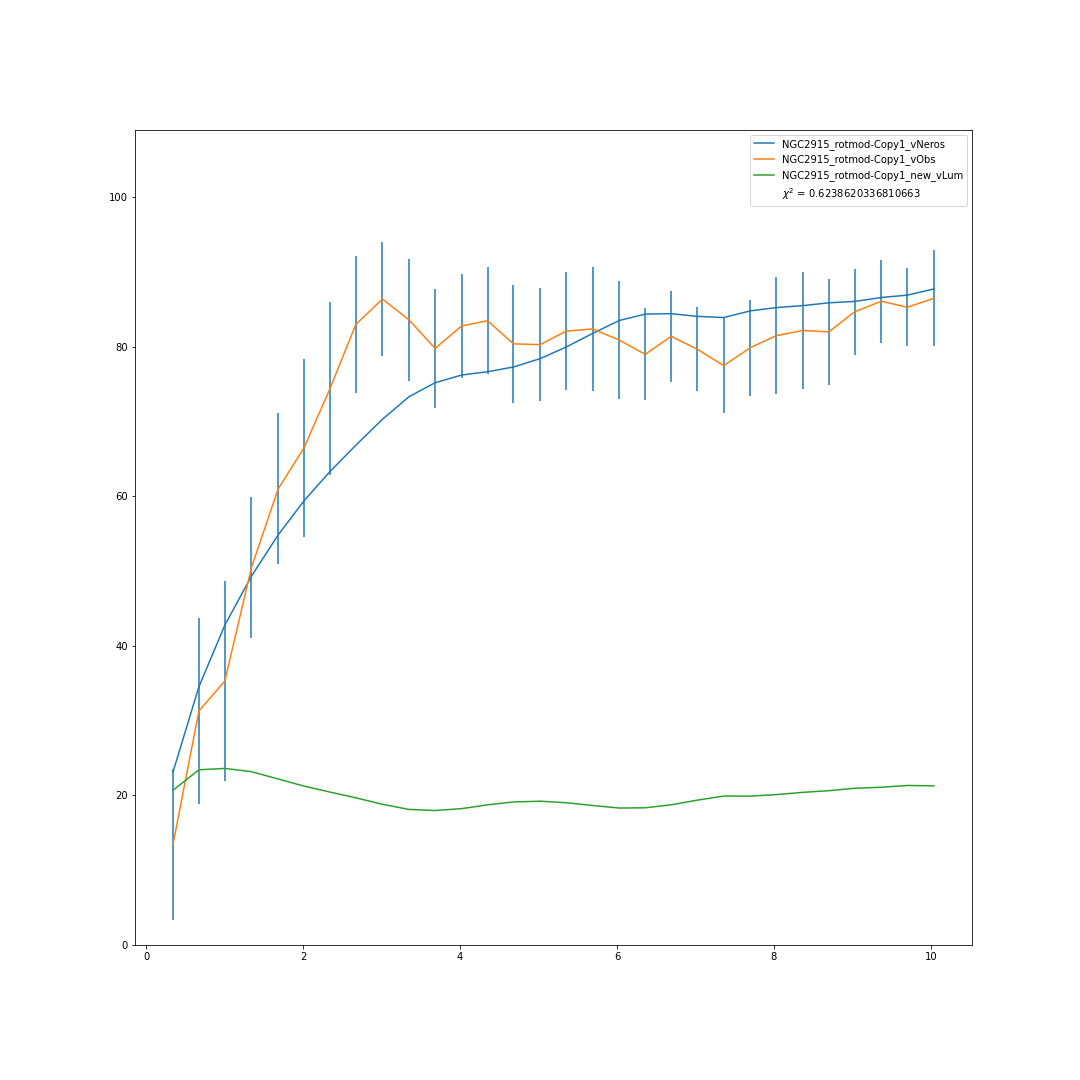
\includegraphics[width=.8\linewidth]{NGC2915_rotmod-Copy1_XueSofue.png}
  \caption{SPARC\cite{2016Lelli}}
  \label{fig:sfig17}
\end{subfigure}%
\begin{subfigure}{.5\textwidth}
  \centering
  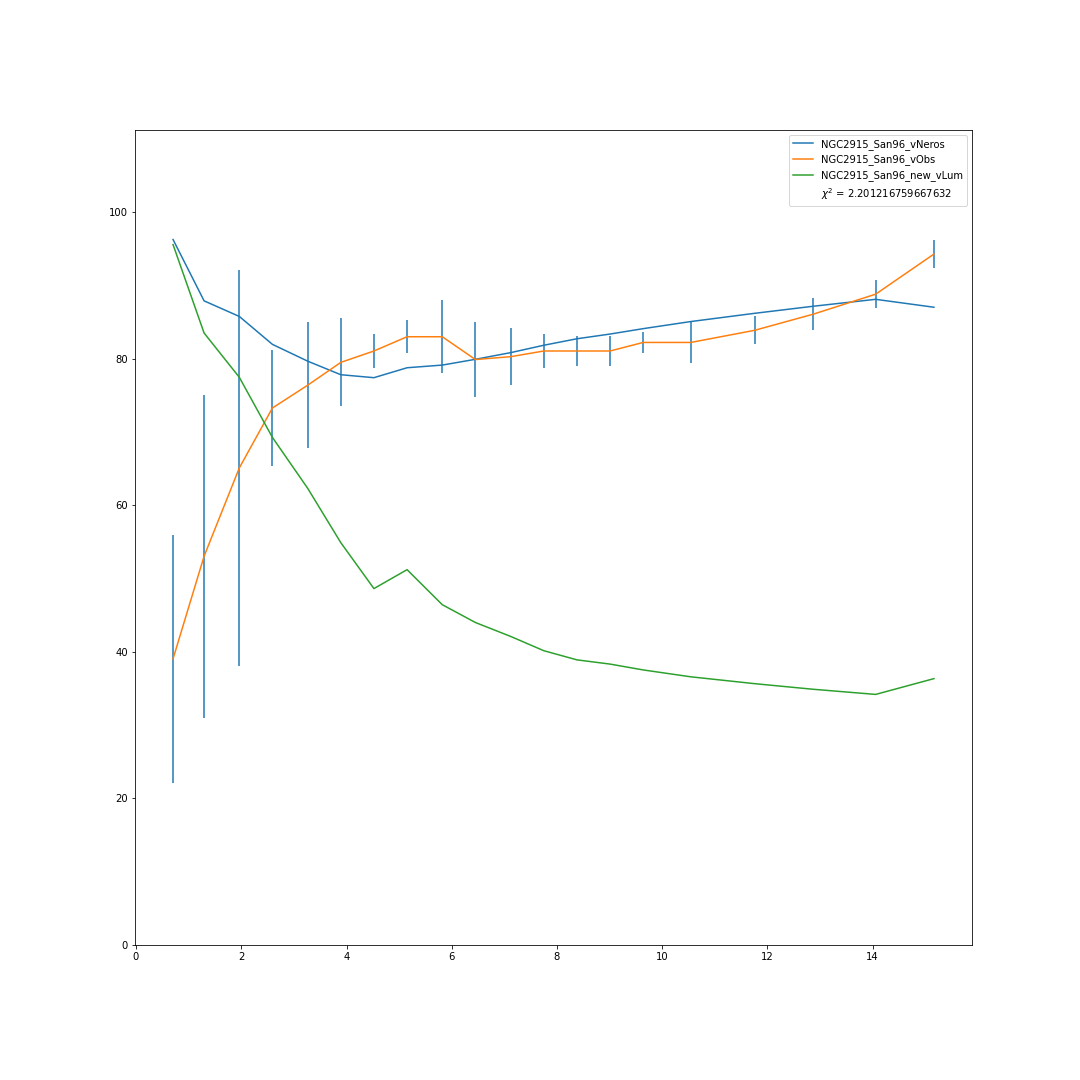
\includegraphics[width=.8\linewidth]{NGC2915_San96_XueSofue.png}
  \caption{Sanders\cite{San96}}
  \label{fig:sfig18}
\end{subfigure}
\caption{plots of NGC 2915}
\label{fig:fig2915}
\end{figure}
%
%
%
%  
%%%%%%%
  \begin{figure}[h]
\begin{subfigure}{.5\textwidth}
  \centering
  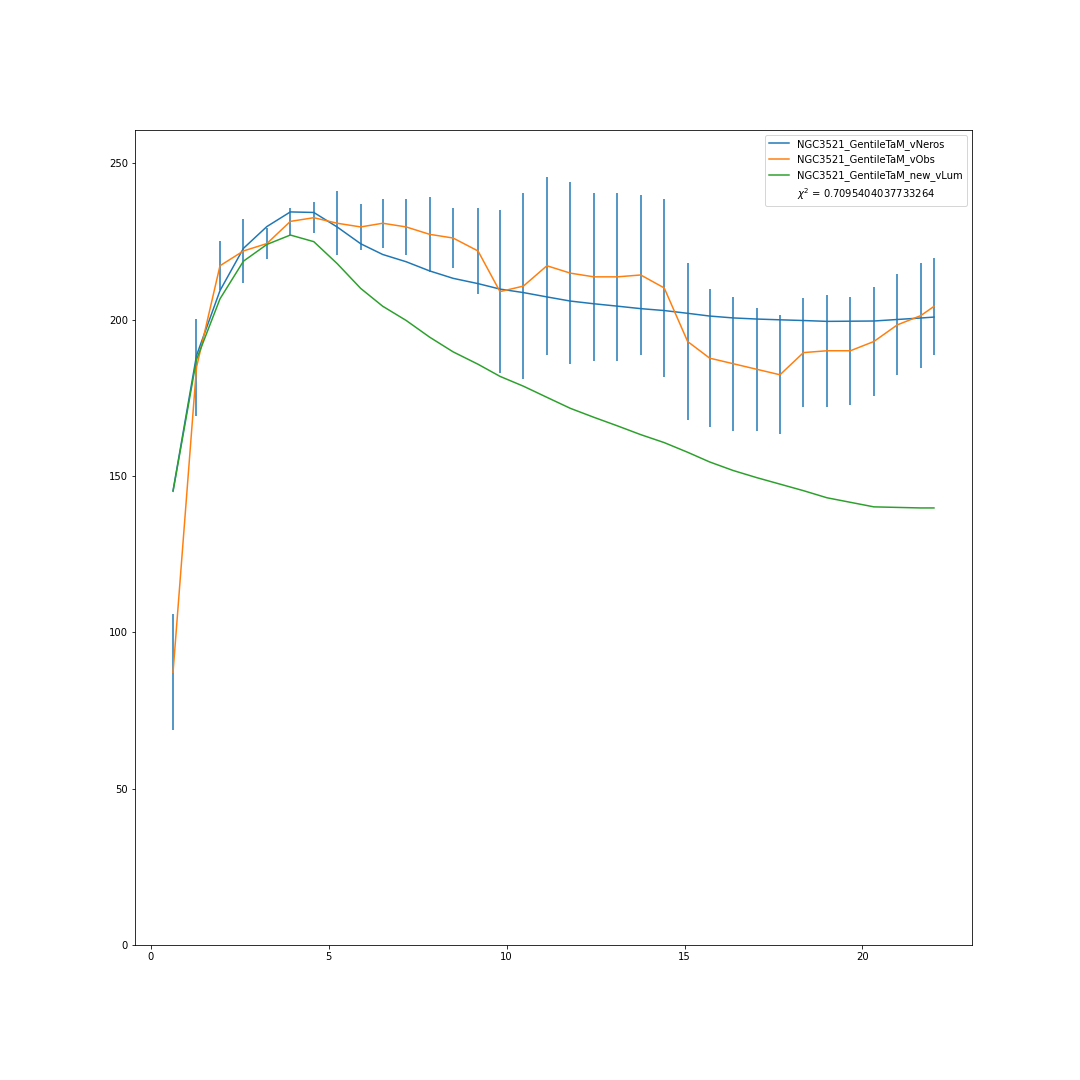
\includegraphics[width=.8\linewidth]{NGC3521_GentileTaM_XueSofue.png}
  \caption{Gentile\cite{Gent}}
  \label{fig:sfig19}
\end{subfigure}%
\begin{subfigure}{.5\textwidth}
  \centering
  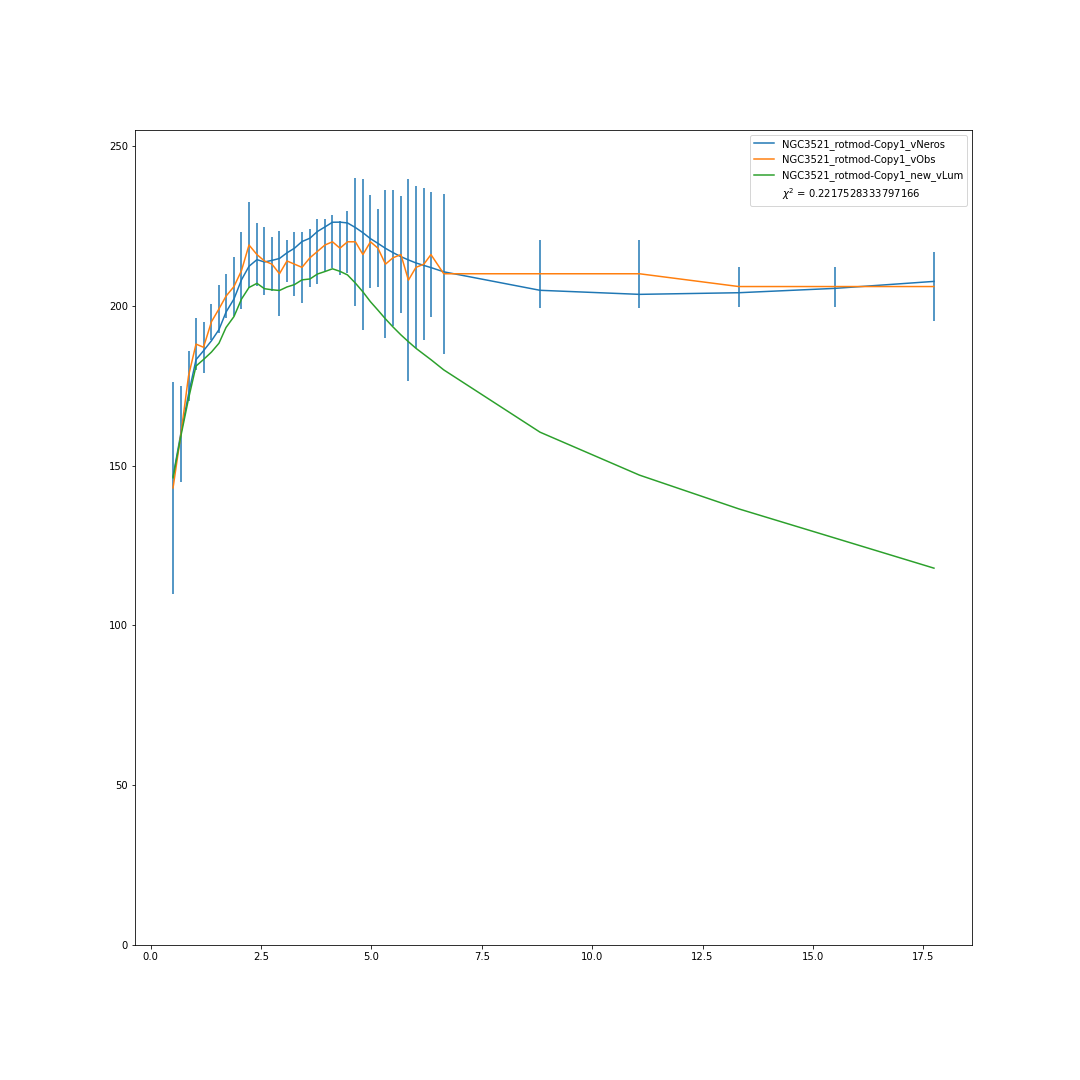
\includegraphics[width=.8\linewidth]{NGC3521_rotmod-Copy1_XueSofue.png}
  \caption{SPARC\cite{2016Lelli}}
  \label{fig:sfig20}
\end{subfigure}
\caption{plots of NGC 3521}
\label{fig:fig3521}
\end{figure}
%
%
%
\clearpage
 \begin{figure}[h]
\begin{subfigure}{.5\textwidth}
  \centering
  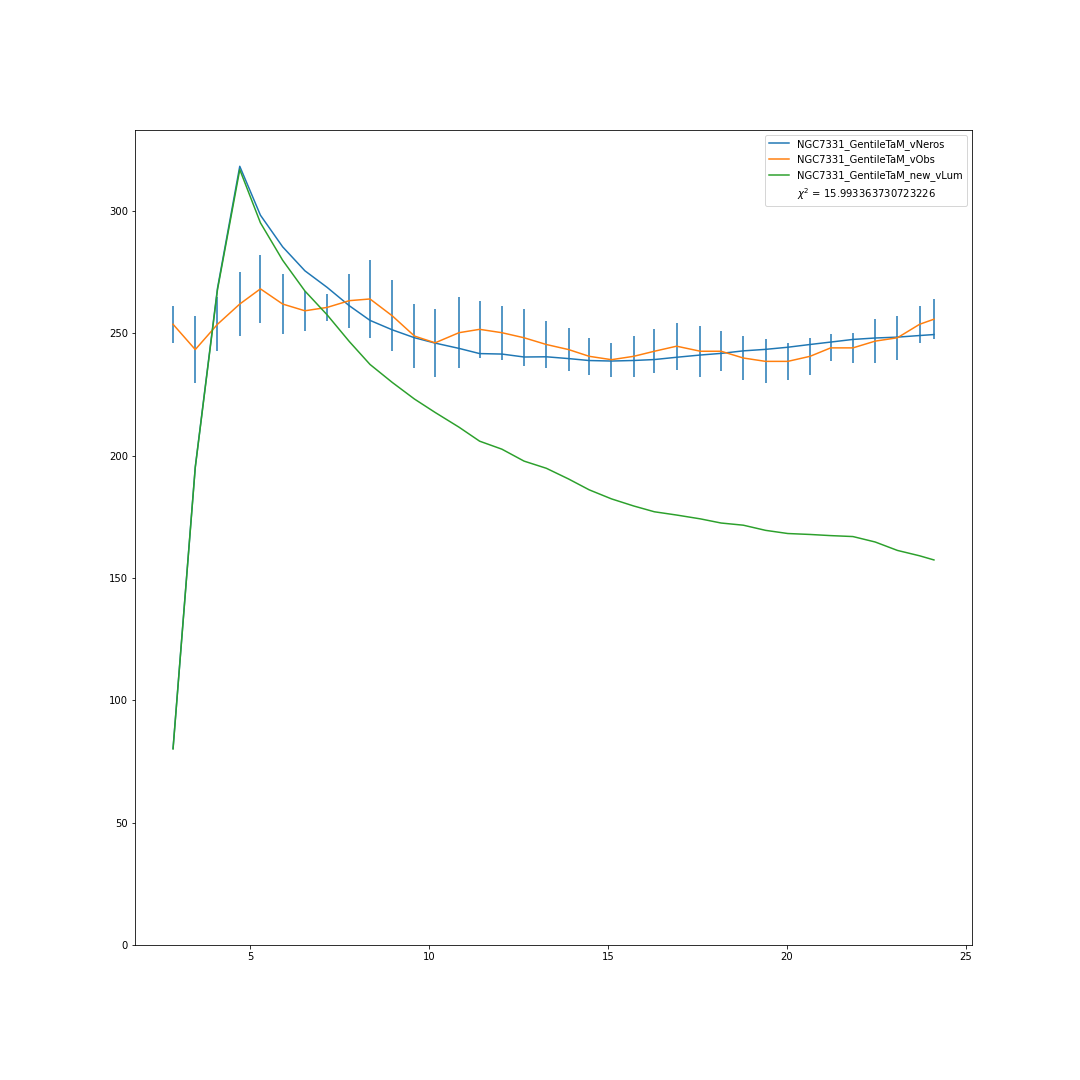
\includegraphics[width=.8\linewidth]{NGC7331_GentileTaM_XueSofue.png}
  \caption{Gentile\cite{Gent}}
  \label{fig:sfig21}
\end{subfigure}%
\begin{subfigure}{.5\textwidth}
  \centering
  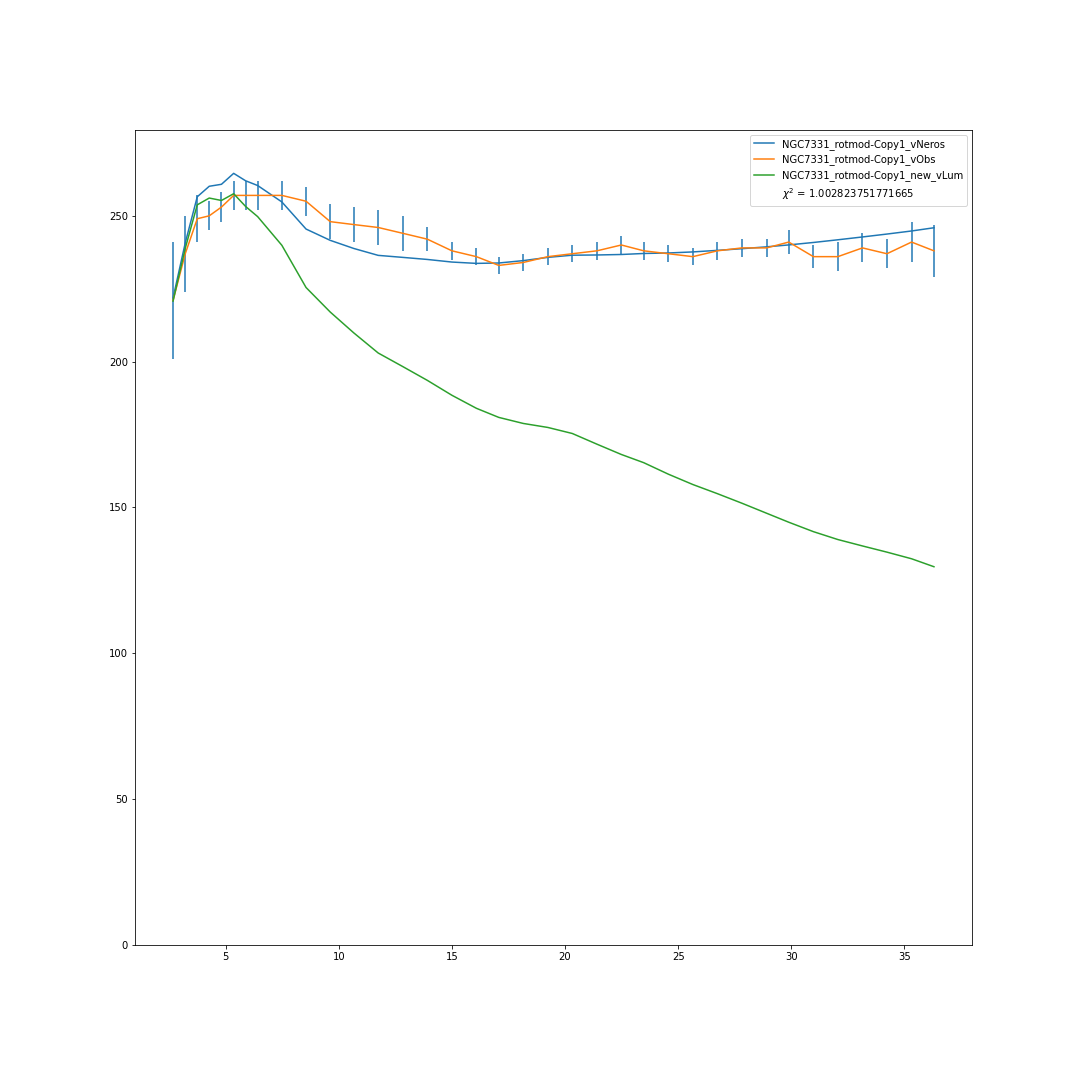
\includegraphics[width=.8\linewidth]{NGC7331_rotmod-Copy1_XueSofue.png}
  \caption{SPARC\cite{2016Lelli}}
  \label{fig:sfig22}
\end{subfigure}
\caption{plots of NGC 7331}
\label{fig:fig7331}
\end{figure}
%%%%%%%
 \begin{figure}[h]
\begin{subfigure}{.5\textwidth}
  \centering
  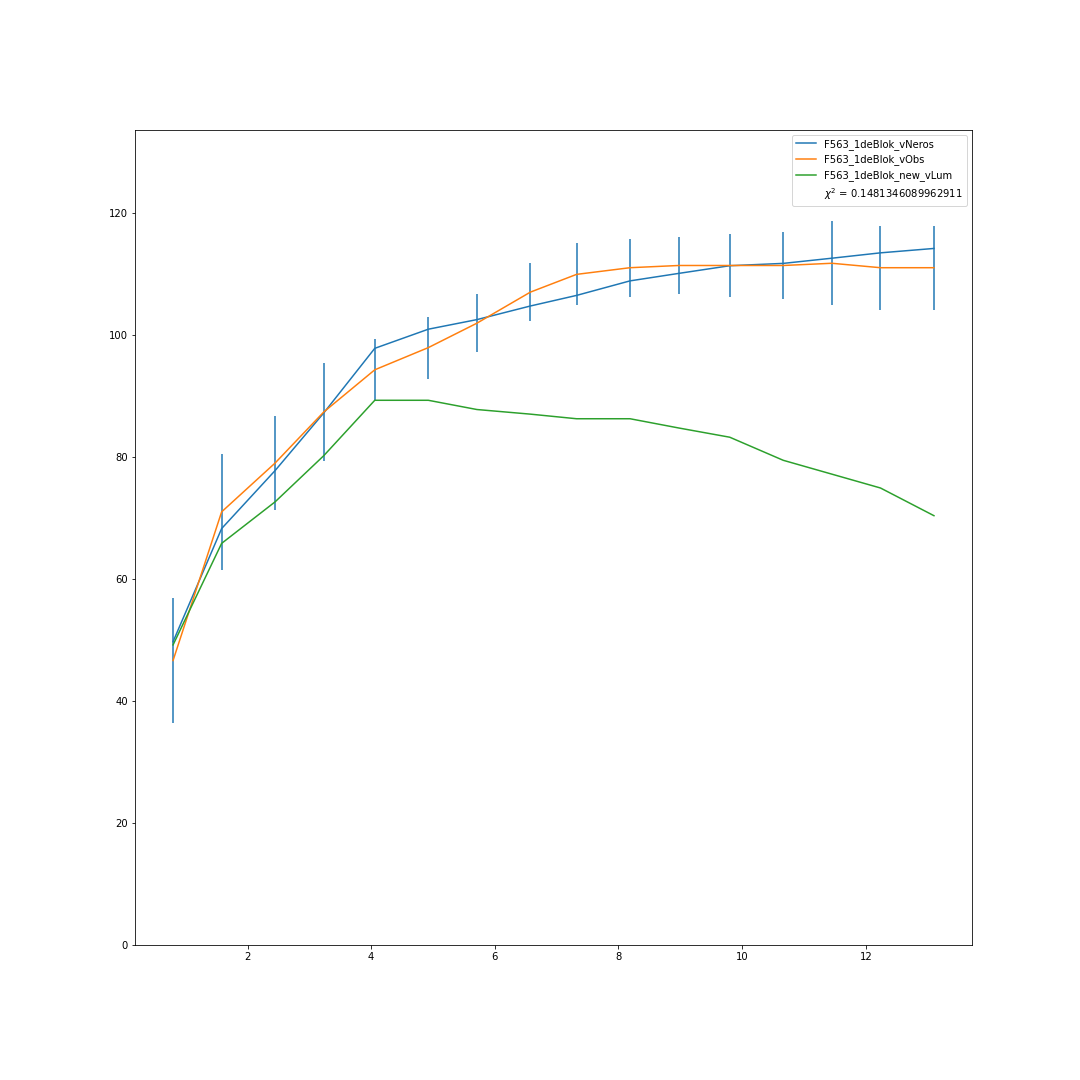
\includegraphics[width=.8\linewidth]{F563_1deBlok_XueSofue.png}
  \caption{de Blok}
  \label{fig:sfig23}
\end{subfigure}%
\begin{subfigure}{.5\textwidth}
  \centering
  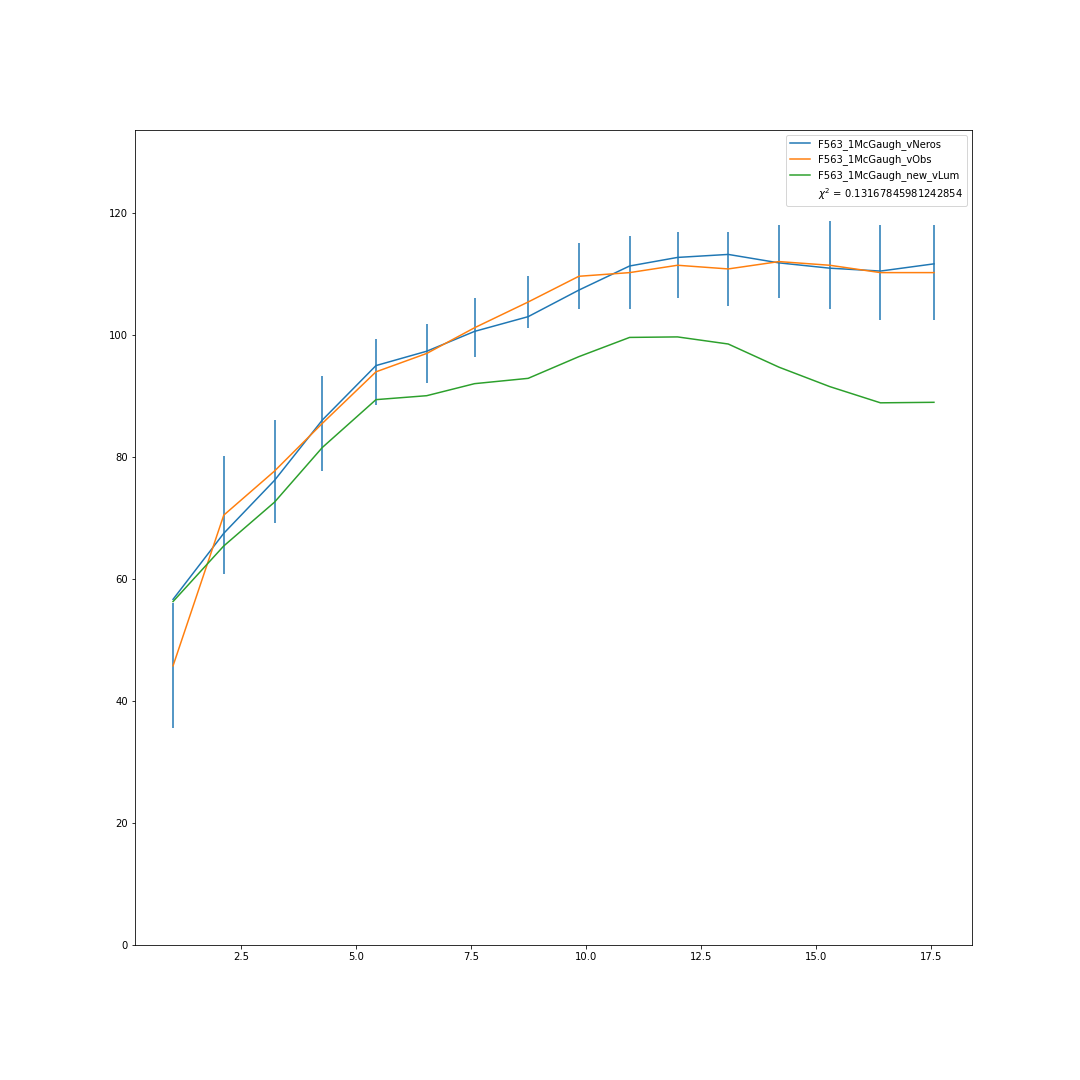
\includegraphics[width=.8\linewidth]{F563_1McGaugh_XueSofue.png}
  \caption{McGaugh}
  \label{fig:sfig24}
\end{subfigure}
\caption{plots of F563-1}
\label{fig:figF563-1}
\end{figure}
\clearpage
%%%%%%
%%%%%%%%
%%%%%%
%%%%%%%
%%%%%%
  
 
\begin{figure*}
    \centering
    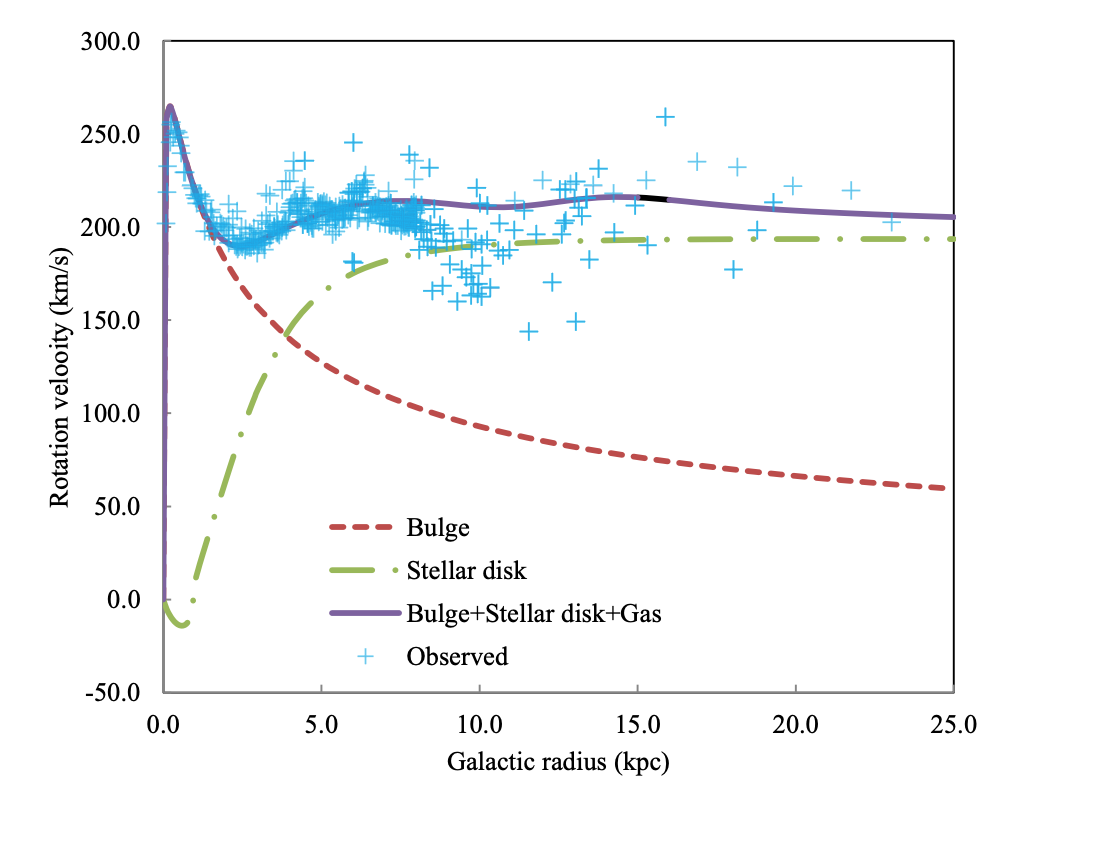
\includegraphics{MW_Enbang_Li}
    \caption{Enbang Li \cite{Li2016ModellingMD}}
    \label{fig:my_label}
\end{figure*}

    
     

\bibliography{LCM} 

\end{document}
%
% ****** End of file apssamp.tex ******